\chapter{Radial time projection chamber}


\section{The EG6 RTPC}

At 6 GeV incident electron beam energy, the recoil $^{4}He$ nuclei from 
the coherent DVCS channel, have an average momentum around 200 MeV/c. CLAS 
cannot detect such low energy particles, for example protons are detected with 
a threshold of about 250 MeV/c, which will be even higher for helium. In order 
to detect such low-energy recoils a Radial TPC (RTPC), similar to the one used 
during the BoNuS run \cite{BONUS}, was added to CLAS. In 2009, the CLAS-EG6 
group \cite{proposal} has built this RTPC, figure \ref{fig:RTPC2} shows a close 
photo of the RTPC, while figure \ref{fig:RTPC_xscetion} shows a schematic 
drawing of its internal structure. It is a 200~mm-long and 150~mm-diameter TPC, 
composed of two electronically separated modules, each covering about 
150$^{\circ}$ of the azimuthal angle. The RTPC tracks the charged particles 
through the ionization centers they leave in the gas-filled detection volume.  
Then, the ionized electrons drift under the effect of an electric field and are 
amplified by a gas electron multiplier system before to be detected on 
collection pads.


\begin{figure}[tp]
\begin{minipage}[c]{.46\linewidth}
\vspace{0.3in}
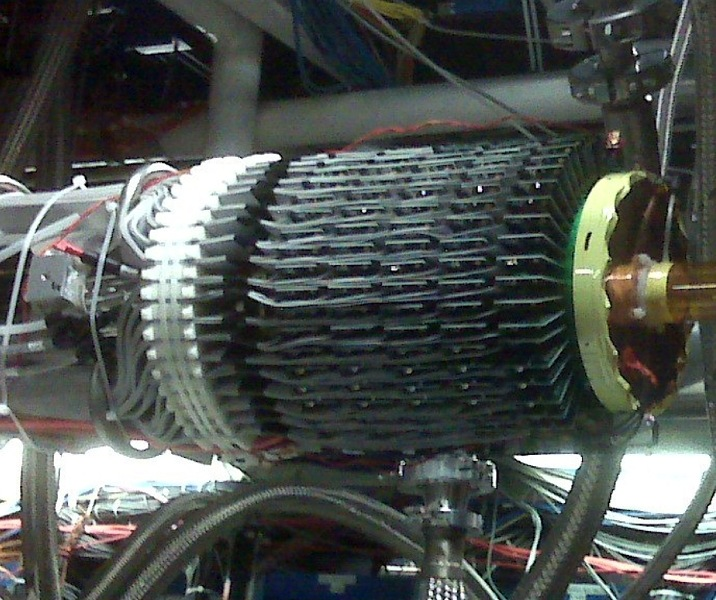
\includegraphics[height=6.2cm]{fig_rtpc/RTPC_exp_cut.jpg}
\vspace{0.1in}
\caption{A view of the RTPC before insertion into the solenoid. The incident 
electron beam comes from the left.} 
\label{fig:RTPC2}
\end{minipage} \hfill
\begin{minipage}[c]{.46\linewidth}
\hspace*{-0.3in}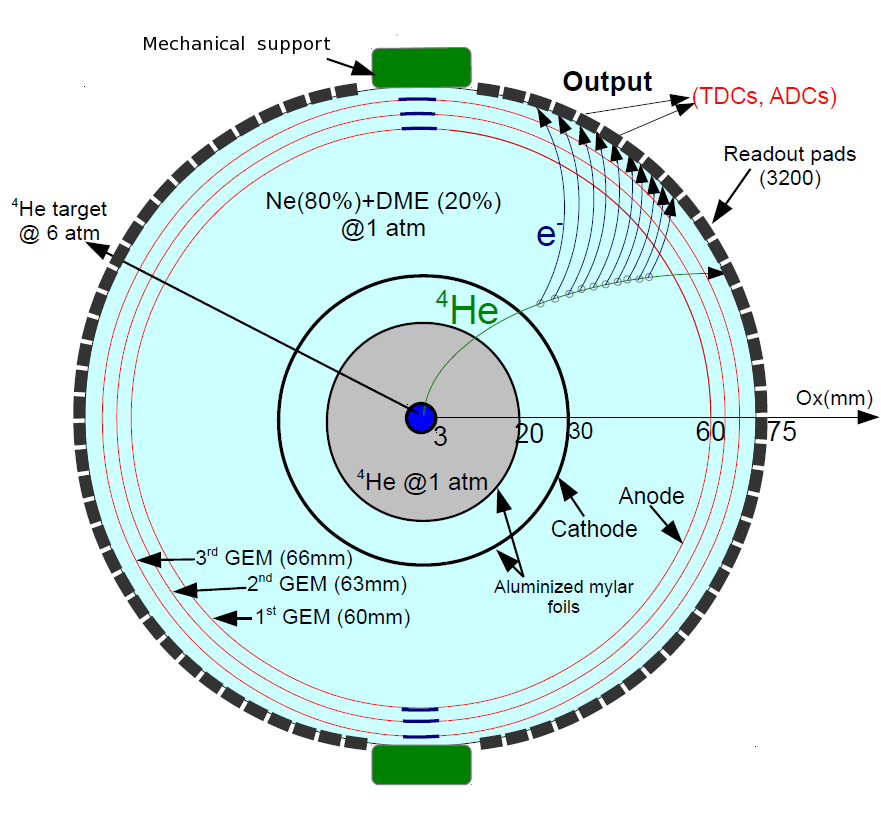
\includegraphics[height=8.0cm]{fig_rtpc/RTPC_1_all.png}
\caption{A cross section of the RTPC taken on a plane perpendicular to the 
beam line, with a typical $^4He$ track crossing the drift volume.}
\label{fig:RTPC_xscetion}
\end{minipage}
\end{figure}


\subsection{Design}

The RTPC has the following substructure, from the beam axis to the exterior:

\begin{itemize}
 \item The target extends along the RTPC's central z-axis, with a diameter of 6 
    mm. It is enclosed in a 27-$\mu$m-thick Kapton wall.

 \item The first gas gap extends from 3 mm to 20 mm radial distances. It is 
    filled with $^{4}He$ gas at one atmospheric pressure. This region is 
    swarmed with M\o ller electrons induced by the beam, but filling this 
    region with a light gas like $^{4}He$ at low pressure minimizes their 
    secondary interactions, while the magnetic field of the solenoid keeps them 
    away from the sensitive drift region. This gap is surrounded by a grounded 
    window made of 4-$\mu$m-thick aluminized mylar.

 \item The second gas gap extends from 20 mm to 30 mm radial distances and is 
    filled with a gas mixture of 80$\%$ Neon (Ne) and 20$\%$ Dimethyl Ether 
    (DME: $C_{2}H_{6}O$). This drift gas fills all the following gaps up to the 
    external shell.

 \item The cathode foil, which is made of 4-$\mu$m-thick aluminized mylar, 
    surrounds the second gas gap. It is connected to a voltage of 4.3 kV to 
    generate an electric field in the drift region.

 \item The drift region is filled with the Ne-DME gas mixture. It extends from 
    the cathode, 30 mm from the beam line, to the first gas electron multiplier 
    layer, 60 mm from the beam line.

 \item The amplification system is composed of three Gas Electron Multiplier 
    (GEM) layers located at radii of 60 mm, 63 mm, and 66 mm.

 \item The electron collection system has an internal radius of 69 mm and 
 collects the charges. The data are then pre-amplified and transmitted to the 
 data acquisition system.  \end{itemize}

The Ne-DME gas mixture has been chosen as the drift gas because of its 
low-diffusion characteristics and small Lorentz angles (the angles between the 
drift direction of electrons under the influence of magnetic field and the 
direction of the electric field). These characteristics minimize the changes in 
the drift velocity of the ionization electrons \cite{DME}. 

The GEMs amplify the ionized electrons to produce measurable signals. Figure 
\ref{fig:GEMs} shows a microscopic photo of a GEM. It is made from an insulator 
(Kapton) sandwiched between two copper layers. The mesh of each GEM layer is 
chemically etched with 50-$\mu$m-diameter holes in double-conical cross section 
shapes, as can be seen from the schematic plot on the right.

\begin{figure}[tbp]
\centering
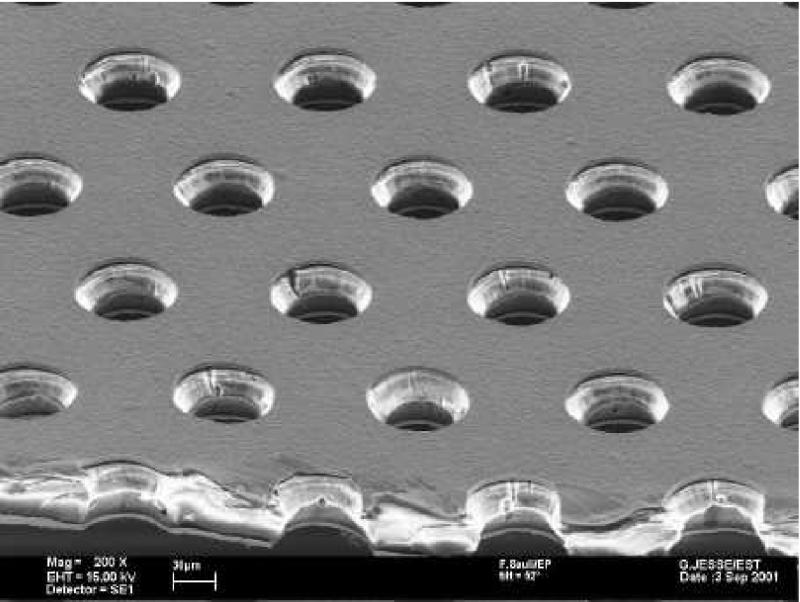
\includegraphics[height=5.5cm]{fig_rtpc/GEM_photo.jpg}
\hspace{0.4in}
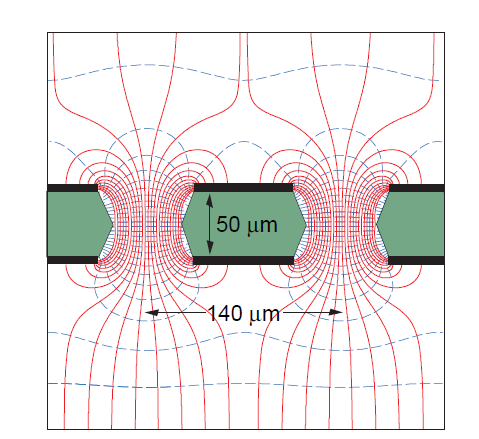
\includegraphics[height=6.0cm]{fig_rtpc/gem_holes.png}
\caption{On the left: A microscopic image of a GEM shows the amplification 
   holes, and the two copper layers, separated by a Kapton insulator. This 
   figure is from \cite{BONUS_2}. On the right: Schematic of the hole structure 
   in the GEMs with the electric field lines (solid red) and the equipotentials 
   (dashed blue). This figure is from
 \cite{GEM_holes}. } 
\label{fig:GEMs}
\end{figure} 


The electrons amplification is achieved through the holes via the strong 
electric field, that is generated by a 400-V potential difference between the 
two copper layers. Such a strong field leads to high ionization of the initial 
electrons and therefore amplification of the signals. Furthermore, an 
additional potential difference of 150 V is set between each two successive GEM 
layers to push the amplified electrons towards the readout board. In this 
configuration, the gain of each GEM layer is of the order of 100.


The RTPC electron collection system has 3200 readout pads. Each module of the 
RTPC has 40 rows and 40 columns of readout pads, each is 5 mm long and 4.45 mm 
wide. Each group of 16 pads is connected to a pre-amplifier before the recorded 
signals are carried to the acquisition electronics. There are 20 rows and 5 
columns of pre-amplifiers per module. This readout system records the charge 
information in time bins, in which the charge is measured in 
Analog-to-Digital-Converter (ADC) units, while the 114 ns width of the time bins 
will be refered as Time-to-Digital-Converter (TDC) units.  
From this measurement, we deduce the time taken by the electrons to drift from the 
ionization point to the readout board.

 
\subsection{Working principle}
When a charged particle traverses a gas, it ionizes the gas-atoms along its 
trajectory. In a TPC, the electrons released in the ionization drift towards 
the readout board under the effect of an applied electric field. The drift 
velocity depends on the gas mixture, and on the electric ($\vec{E}$) and 
magnetic ($\vec{B}$) fields. The recorded time of the electrons provides 
information on how far the initial ionizations happened in the drift region, 
leading to reconstruct the original points of ionization, while the recorded 
ADCs give the deposited energy.

In our TPC the cathode and the anode are two cylinders. Thus, the generated 
$\vec{E}$ field in the drift region has a purely radial components, 
perpendicular to the beam line, with a magnitude around 500 V/cm. However, the 
two-cylinders configuration produces small gradient components at the sides of 
the RTPC. This issue was solved by installing field cages at the ends of the 
RTPC to keep a regular $\vec{E}$ field. These caused some high voltage issues 
and were disconnected during the experiment, partly justifying the time 
dependent calibration described below. 

The $\vec{B}$ field is generated by the solenoid. Figure \ref{fig:B_MAP} shows 
the magnetic field vectors in the different regions of the RTPC. The presence 
of the magnetic field enables us to deduce the momentum of a charged particle 
from the curvature of its track and the known magnetic field.
% from:
%\begin{equation}
%p = R q |\overrightarrow{B}| sin(\theta)
%\end{equation}
%where R is the radius of the track's curvature, q and $\theta$ are the charge 
%and the polar angle of the %particle.

\begin{figure}[tp]
\centering
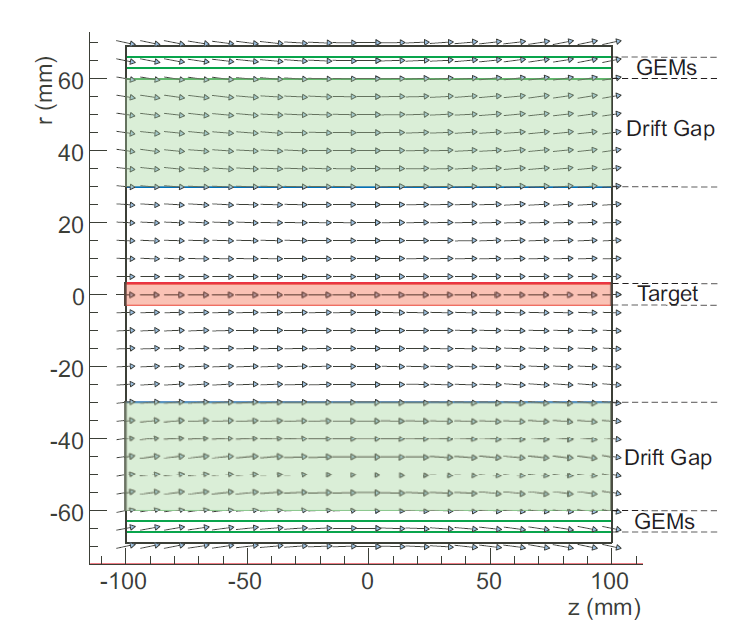
\includegraphics[scale=0.40]{fig_rtpc/B_MAP.png}
\caption[]{The solenoid magnetic field vectors in the RTPC, shown in the $r-z$ 
plane, where $r$ is the radial distance from the central axis and $z$ 
represents the longitudinal distance along the RTPC.} \label{fig:B_MAP}
\end{figure}

\subsection{Track reconstruction}
In order to reconstruct tracks we must first select the good hits. The 
first step is the rejection of out-of-time hits and the noise reduction, as 
will be explained in section \ref{sec:noise_rejection}. The second step is the 
spatial reconstruction of the hits, using the extracted drift speed and drift 
paths. For each registered hit, the position of the initial ionization is 
obtained from the recorded time (TDC) and from the position of its pad. In the 
third step, the reconstructed nearby hits are linked together in chains. The 
maximum distance between two adjacent hits must be less than 10.5 mm to chain 
them. Then, the number of hits per chain is required to be greater than 10 hits 
in order to proceed to the fitting step. 

A fit to a chain of hits is performed in two iterations. In the first 
iteration, the hits of the chain are fitted with a helix. The helix fit is 
based on a circle fit in the $x-y$ plane followed by a linear fit in the $s-z$ 
plane for the hits of the chain, where $s=\sqrt{x^2+y^2}$. In the second 
iteration, the residual between the fit and each hit is calculated. If the 
hit's residual is greater than 5 mm, the hit is excluded from the chain. Then 
the hits are re-fitted with the same previous helix fit giving five final 
parameters for each track's chain. From these five parameters, one can 
reconstruct all the parameters of a track. For example, one can calculate the 
momentum from the known longitudinal magnetic field ($\vec{B_{z}}$), the radius 
of curvature of the track ($r_{0}$) and the polar angle ($\theta$), like:
\begin{eqnarray}
p_{tot} = \sqrt{p_{\|}^2 + p_{\perp}^2}, ~~~~~~~~~~~~~~~~~~~~~~~~~~~~~~~~~~~~~~~ \\
\text{with } p_{\perp} = 0.3\cdot q \cdot B_{z} \cdot |r_{0}|\text{and } p_{\|} 
= p_{\perp}/tan(\theta),\nonumber
\end{eqnarray}
where $p$ is in GeV/c unit, $q$ is the elementary charge, $B_{z}$ is in Tesla 
(T) and $r_{0}$ is in meters (m). For example, In a magnetic field of 4.5 T, 
the recoil $^4$He nuclei from DVCS (elastic) reaction have kinetic energies in 
the range [10, 25] ([17, 35]) MeV, from momenta of [260, 450] ([360, 550]) MeV 
and $r_{0}$ [70, 150] ([130,180]) mm.


\section{RTPC calibration}
Reconstructing a trajectory from the recorded time information of the 
electrons requires a good knowledge of their drift speed and drift paths.  
Also, the gains of the readout pads are required to calculate $\frac{dE}{dx}$ 
from the recorded ADCs. The determination of the drift paths and the gain 
calibration of the RTPC 
require well identified events, so we decided to use elastic scattering 
($e^{4}He \rightarrow e^{4}He$). However, the cross section of 
the elastic process at detectable angles is highly suppressed at higher beam 
energy, so we had specific calibration runs with 1-pass 
beam energies of 1.024 and 1.269 GeV.

A GEANT4 simulation for the RTPC has been developed to help reproduce these 
events in order to properly extract the drift paths and the gains. Their 
extractions are based on comparing the experimentally identified $^4He$ elastic 
tracks to the GEANT4 simulated ones. Indeed, the kinematics of each elastic 
$^4He$ can be calculated from the electron measured in CLAS and then simulated 
in GEANT4. The output of the simulation gives an expected trajectory that we then
match to to the measured signals to determine the drift paths. 

This process is iterative since good tracks need to be identified at the 
beginning of the process and as the calibration improves, more good tracks 
are identified. For this analysis, we started from a MAGBOLTZ 
calibration, which was then improved with the method described above with 
several iterations. In particular, it is important that the alignment of the 
RTPC with respect to the beamline is properly implemented (see details in
CLAS-NOTE~\cite{eg6beamoffset}). As the process evolved and was improved over 
time, we present in the following subsections only the method used for the last 
iteration of our calibration process.

\subsection{Event selection}
Figure \ref{fig:RTPC_track} shows a drawing of a segment of the RTPC, 
where a $^4He$ track (in 
green) crosses the volume of the RTPC, producing a chain of ionization points 
within the drift gas. The released electrons follow the drift paths (in black) 
towards the readout board under the effect of the electromagnetic field 
between the anode and the cathode. The electrons released close to the cathode 
take the maximum drift time ($TDC_{max}$) to reach the readout pads, while the 
electrons released close to the anode take the minimum time ($TDC_{min} = 15$ the 
trigger time), also called time offset, which is identical 
for all readout channels. In our convention, the distance between the 
first ionization point in the chain and the cathode is labelled as $sdist$, 
while the distance between the last point and the anode is labelled as 
$edist$. 

\begin{figure}[tbp]
\centering
\vspace{-0.1in}
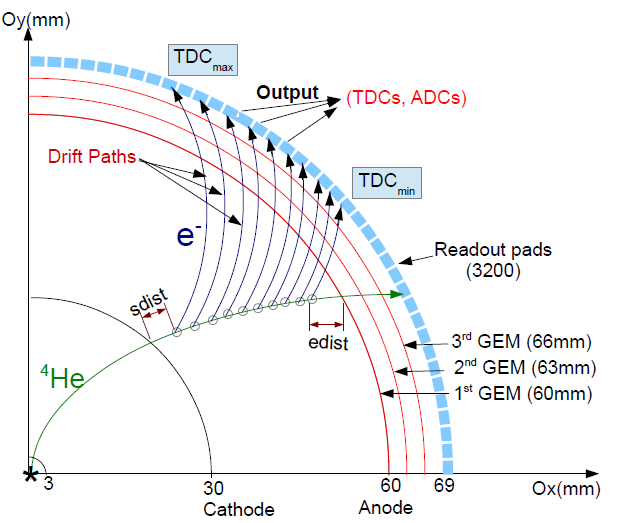
\includegraphics[scale=0.38]{fig_rtpc/RTPC_track.png}
\vspace{-0.1in}
\caption{Schematic of a segment of the RTPC in a plane perpendicular to the 
beam line, with a $^4He$ track (in green) crossing the volume. See the text for 
description of the various elements and notations. $sdist$ and $edist$ are 
distances between first and last hits and boundaries of the RTPC as shown in 
this sketch.} \label{fig:RTPC_track}
\end{figure}

Because the two modules of the RTPC are electronically separated, we will 
sometimes show their distributions separately. In our angular convention, the 
right module of the RTPC covers the azimuthal angles between 90$^{\circ}$ and 
270$^{\circ}$, while the left-side module covers the rest of the azimuthal 
angles. 

\subsubsection{RTPC good track requirements} \label{good_track_req}

A good RTPC track passes the following requirements:
\begin{itemize}
\item The number of active pads in the track is greater than 3. 

\item The vertex position in $z$ is in the RTPC volume, i.e. $z$ $\in$ [-80,80] mm, as 
   illustrated in figure \ref{fig:rtpc_zz}.  

\item The radius of curvature is positive ($r_{0}>0$): the $^4He$ is a positively 
   charged nucleus and the reconstructed track in the RTPC must have positive 
   radius of curvature. In other words, it travels in a clockwise direction if 
   one looks into the electron beam. The curvature distribution of the 
   collected RTPC tracks is shown in figure \ref{fig:rtpc_ro}.

\item The helix fit is well reconstructed with a $\chi^{2} < 3.5$. The 
   quality of the fit ($\chi^{2}$) being defined as:
\begin{equation}
   \chi^{2} = \frac{\displaystyle \left(\frac{DOCA}{\sigma_r}\right)^2 
       + \sum_{i = 1}^{ N_{pts}} \left(\frac{r^{pt}_{i} 
      - r^{helix}_{i} }{\sigma_{r}}\right)^{2}  + \left( \frac{\phi^{pt}_{i} - 
      \phi^{helix}_{i} }{\sigma_{\phi}}\right)^{2} + \left( \frac{z^{pt}_{i} - 
   z^{helix}_{i} }{\sigma_{z} } \right)^{2}}{N_{pts} - 4}
\end{equation}
where $\frac{DOCA}{\sigma_r}$ is the beam-spot constraint, $r^{pt}_{i}$, 
$\phi^{pt}_{i}$, $z^{pt}_{i}$ are the radial, azimuthal, longitudinal 
coordinates of each reconstructed hit "$i$". ($r^{helix}_{i}$,
$\phi^{helix}_{i}$, $z^{helix}_{i}$) is the point on the helix fit that is 
closest to the reconstructed hit $i$. The resolutions 
are defined as ($\sigma_{r}$, $\sigma_{\phi}$, $\sigma_{z}$) = (0.53 mm, 
2$^{\circ}$, 1.2 mm) based only on the size
of the readout pads and were kept identical for all calibration iterations. These 
resolutions were derived by CLAS-BoNus experiment \cite{BONUS}. $N_{pts}$ is 
the total number of the hits in the chain. Figure \ref{fig:rrtpc_X2} shows the 
$\chi^{2}$ distributions for the positive tracks which originate within the 
RTPC.

\begin{figure}[tbp]
\centering
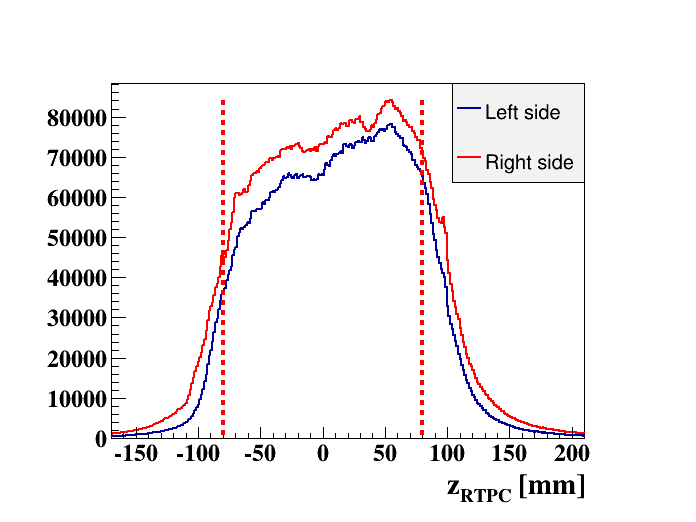
\includegraphics[scale=0.38]{fig_rtpc/rtpc_z.png}
\caption{The z-vertex distributions for the reconstructed tracks in the RTPC.} 
\label{fig:rtpc_zz}
\end{figure}  

\item $sdist$ ($\in$ [-2.0,2.0] mm) and $edist$ ($\in$ [-1,5] mm ): these 
   cuts are applied to ensure that a track is on time, i.e. the first 
   ionization point is close to the cathode and the last point is close to the 
   anode. For both $sdist$ and $edist$, positive values correspond to tracking 
   points inside the drift region, while negatives are outside the drift 
   region. So, in terms of the path length of the track starting from the 
   vertex, $sdist$ and $edist$ have opposite signs. The $sdist$ and $edist$ 
   distributions are shown in figures \ref{fig:rrtpc_sdist} and 
   \ref{fig:rrtpc_edist} respectively\footnote{The long tail on the positive 
      side of the $edist$ distribution is mostly due to electronic noise.  Note 
      that after applying all the elastic He-4 selection cuts, we observe that 
   most of the tails for both $edist$ and $sdist$ are removed.}. 

\item Vertex correspondence: the track reconstructed in the RTPC has to 
   originate from the same place as the electron that triggered the event. We 
   define $\Delta z$ as the difference between the electron z-vertex and the 
   z-vertex of the RTPC track. Due to variations in the electric and the 
   magnetic fields along the 200 cm of length of the RTPC, $\Delta z$ shows a 
   dependence on the longitudinal position along the RTPC ($z_{RTPC}$). This 
   can be seen in figure \ref{fig:rrtpc_delta_z}. These distributions are 
   fitted to extract the mean and the width of $\Delta z$ as a function of 
   $z_{RTPC}$. We then apply a 2$\sigma$ cut around the mean to select the RTPC 
   good tracks. The parametrizations of the mean ($\mu$) and the width 
   ($\sigma$) of $\Delta z$ can be found in Appendix \ref{app:RTPC_appendix}.

\begin{figure}[tbp]
\begin{minipage}[c]{.46\linewidth}
\hspace{-0.3in}
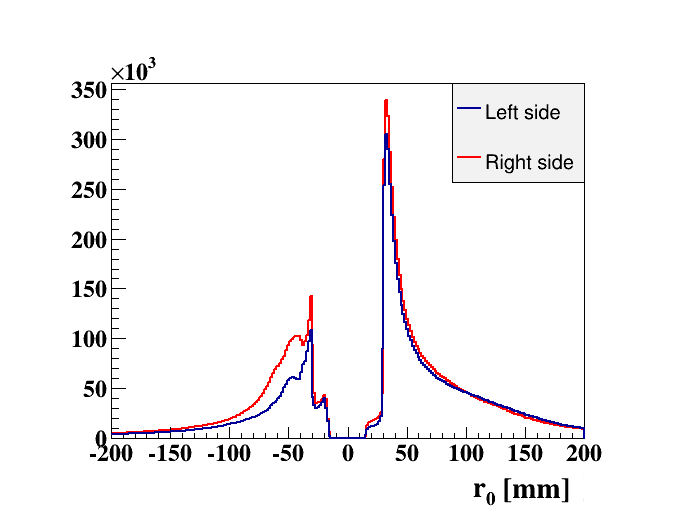
\includegraphics[height=6.5cm]{fig_rtpc/rtpc_r0.png}
\caption{The radius of curvature of the reconstructed tracks in the RTPC.} 
\vspace{0.4in}
\label{fig:rtpc_ro}
\end{minipage} \hfill
\begin{minipage}[c]{.46\linewidth}
\hspace{-0.3in}
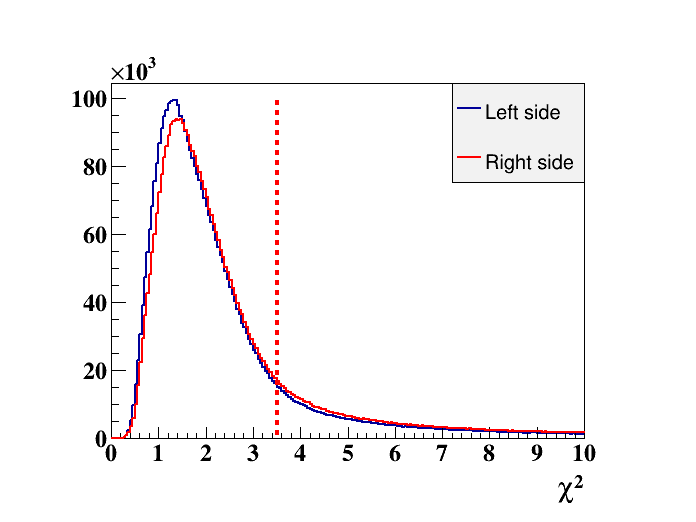
\includegraphics[height=6.5cm]{fig_rtpc/rtpc_X2.png}
\caption{The $\chi^{2}$ distribution for the positive tracks in the RTPC. The red 
line represents the cut we apply to select good tracks.}
\vspace{+0.1in}
\label{fig:rrtpc_X2}
\end{minipage}
\end{figure}

\begin{figure}[tbp]
\begin{minipage}[c]{.46\linewidth}
\hspace{-0.3in}
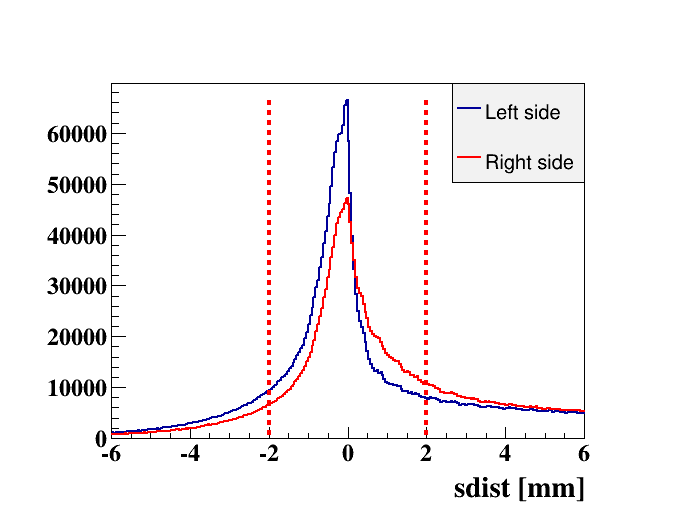
\includegraphics[height=6.5cm]{fig_rtpc/rtpc_sdist.png}
\caption{$sdist$ distribution for the positive tracks in the RTPC. We set $|sdist| < 2.0$ mm to select good tracks.} 
\vspace{0.3in}
\label{fig:rrtpc_sdist}
\end{minipage} \hfill
\begin{minipage}[c]{.46\linewidth}
\hspace{-0.3in}
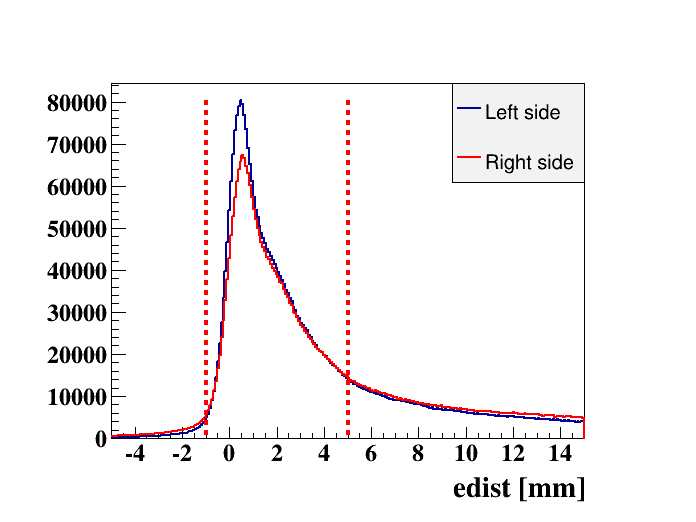
\includegraphics[height=6.5cm]{fig_rtpc/rtpc_edist.png}
\caption{$edist$ distribution for the positive tracks in the RTPC. We require -1.0 mm < $edist$ < 5.0 mm to select the good tracks.}
\vspace{+0.2in}
\label{fig:rrtpc_edist}
\end{minipage}
\end{figure}


\begin{figure}[tbp]
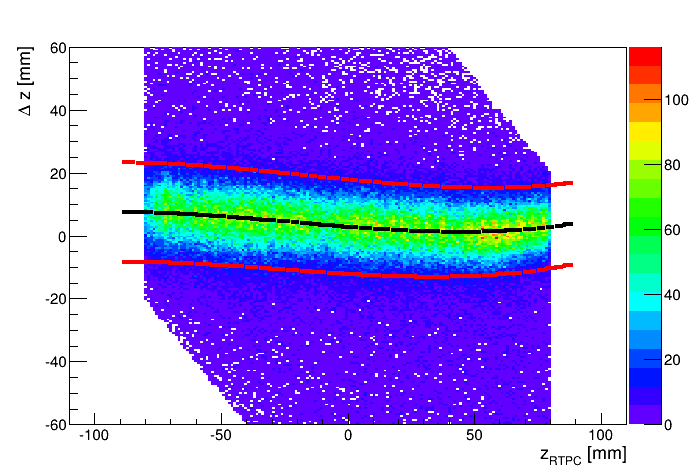
\includegraphics[scale=0.34]{fig_rtpc/delta_z_z_l.png}
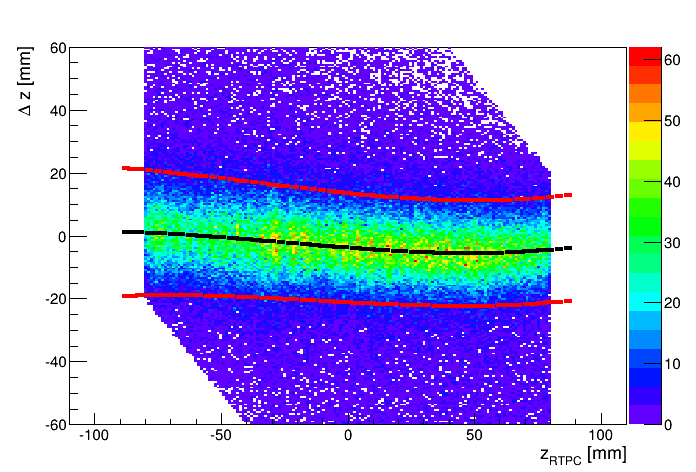
\includegraphics[scale=0.34]{fig_rtpc/delta_z_z_r.png}
\caption{The $\Delta z$ distribution versus the RTPC longitudinal position ($z_{RTPC}$) for the left and the right modules of the RTPC, respectively. The black lines represent the mean value of $\Delta z$ as a function of $z_{RTPC}$, while the red lines are 2$\sigma$ cuts around the mean.} 
\label{fig:rrtpc_delta_z}
\end{figure}  
\end{itemize}


\subsubsection{Elastic scattering event selection}
   The elastic process on $^{4}He$ is defined as:
\begin{equation}
\centering
e(k) + ^{4}He(p) \rightarrow e(k') + ^{4}He(p')
\end{equation}
with the symbols in parenthesis representing the four-momenta of the particles. 

 In addition to the good-track requirements described above, to select elastic events we impose further constraints. The co-planarity between the scattered electron and the recoil $^4He$ is ensured using a $\Delta \phi$ (=$\phi_{e}-\phi_{^{4}He}$) cut as shown in Figure \ref{fig:delta_phi_elastic}. Like for $\Delta z$, the $\Delta \phi$ 2$\sigma$ cut is dependent on $z$ to account for systematic variations. Our final parametrizations can be found in Appendix \ref{app:RTPC_appendix} as well.

An additional elastic cut is performed by comparing the measured $^4He$ polar angle to the calculated one, based on the measured electron in CLAS. Indeed, from momentum conservation the $^4He$ polar angle can be calculated as:
\begin{eqnarray}
\theta^{^4He}_{cal} &=&  sin^{-1}\left(\frac{p_{e'}}{p^{^4He}_{cal}} \cdot \sqrt{1-cos^{2}\theta_{e'}}\right) \\
\text{ with~~} p^{^4He}_{cal} &=& \sqrt{(E_{b} + M_{^4He} - p_{e'})^{2} - M^{2}_{^4He}}
\label{equ:theta_helium}
\end{eqnarray}
where $p_{e'}$ and $\theta_{e'}$ are the electron's measured momentum and polar angle, $E_{b}$ is the beam energy and $M_{^4He}$ is the helium mass (3.727 GeV/c$^{2}$). Figure \ref{fig:delta_theta_elastic} shows the $\Delta \theta$ ($\theta^{^4He}_{cal}$ - $\theta^{^4He}_{meas}$) distribution versus the $^4He$ z-vertex. No significant difference was observed between the two modules regarding this quantity. The obtained parametrization of the mean and the width of the $\Delta \theta$  distribution can be found in Appendix \ref{app:RTPC_appendix}.

\begin{figure}[tp]
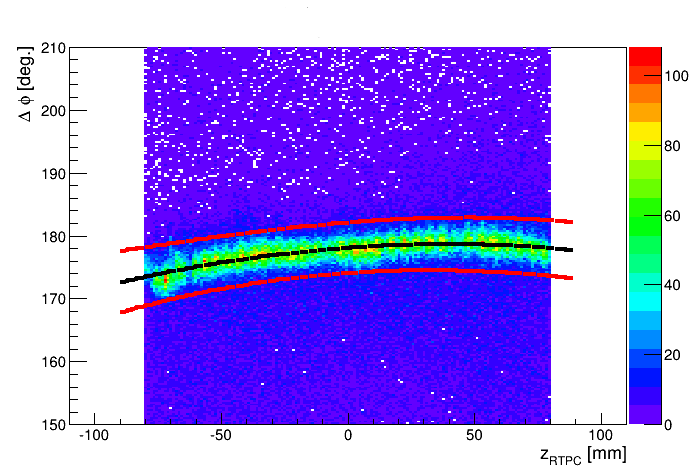
\includegraphics[scale=0.34]{fig_rtpc/delta_phi_z_l.png}
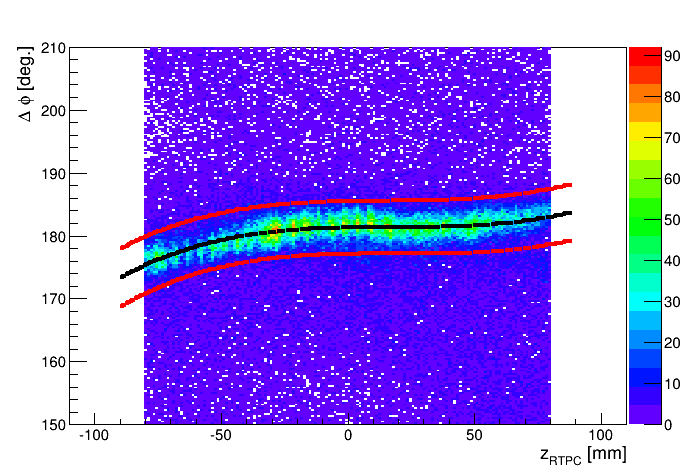
\includegraphics[scale=0.34]{fig_rtpc/delta_phi_z_r.png}
\caption[]{The distributions of $\Delta \phi$ as a function of $z$ along the RTPC for the selected good tracks in the RTPC, for the two halves of the RTPC respectively. In each plot, the black line is the mean of $\Delta \phi$ and the red lines are 2$\sigma$ cuts to select the elastic events.} 
\label{fig:delta_phi_elastic}
\end{figure} 

\begin{figure}[tbp]
\centering
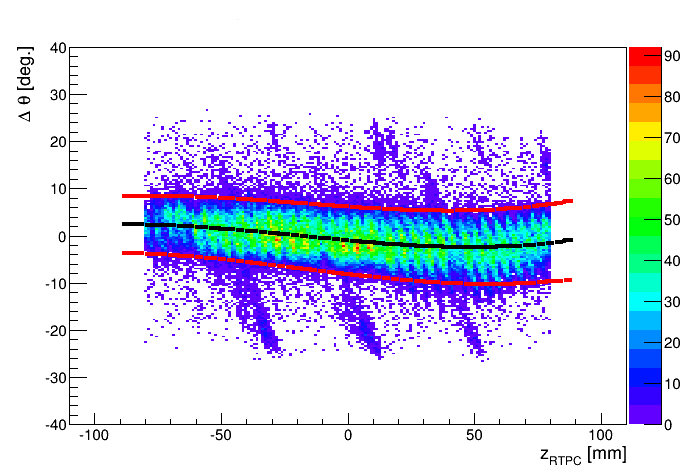
\includegraphics[scale=0.370]{fig_rtpc/delta_theta_z.png}
\caption[]{The $\Delta \theta$ distribution, for the selected events after the $\Delta \phi$ cut, as a function of $z$ along the RTPC. The black line represents the mean, while the red lines are 2$\sigma$ cuts around the mean to select the elastic $^4He$ events. } 
\label{fig:delta_theta_elastic}
\end{figure} 


Constructing the invariant mass is one way to verify the efficiency of the previously described selection procedures. For a helium target, the invariant mass (W) is:
\begin{equation}
 W = \sqrt{-2E_{b}p_{e^{'}}(1-cos(\theta_{e^{'}})) + M_{^{4}He}^2 + 2(E_{b}-p_{e^{'}}) M_{^{4}He}}.
\end{equation}
with the conventions for the variables as in equation \ref{equ:theta_helium}.  
Figure \ref{fig:W_elastic} shows the W distribution of the events that have a 
good track in the RTPC and the identified elastic events. One can see the good 
agreement between the helium-4 real mass and the mean value of the identified 
elastic events. The difference in width is related to differences in 
resolution in CLAS.
The large effect is due to the reaction products being emitted back to 
back resulting in a small overall acceptance for the process. This result is
therefore very sensitive to the local 
variations of the resolution, which can be rather important in CLAS.

\begin{figure}[tbp]
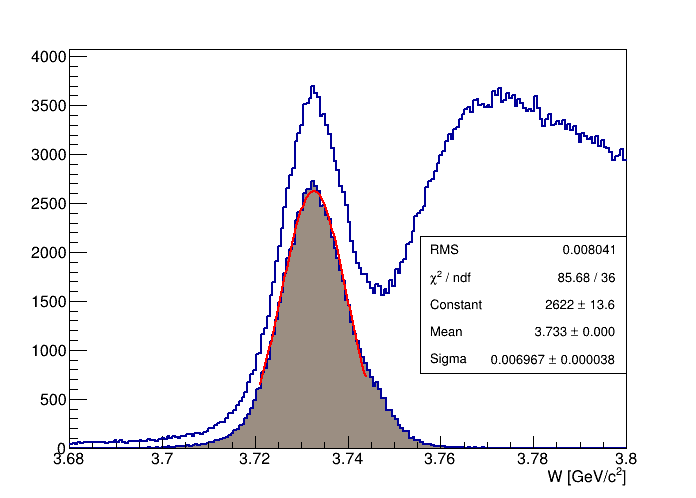
\includegraphics[scale=0.32]{fig_rtpc/fit_W_distribution_l.png}
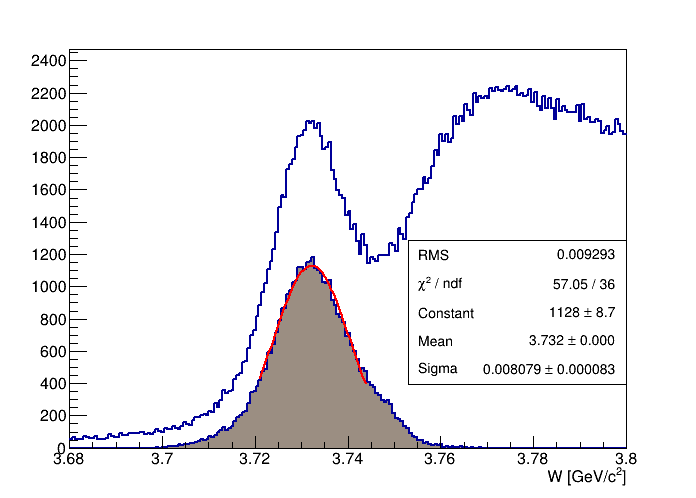
\includegraphics[scale=0.32]{fig_rtpc/fit_W_distribution_r.png}
\caption[]{The invariant mass distributions for events with one good RTPC track (in blue) and the events passing the elastic cuts (in shaded) for each of the two modules of the RTPC, respectively.}
\label{fig:W_elastic}
\end{figure}

The figures presented for $\Delta z$ and $\Delta\phi$ distributions in this section are shown after all the
calibration and detector alignments (RTPC alignment is described in 
CLAS-NOTE-2013-008). The observed remaining dependences are not fully 
understood and probably arise from field misalignement and variations in the 
electric and magnetic fields within the chamber.


\subsubsection{Checking the initial good track requirements}
In this section, we study some of the good track requirements 
presented in section \ref{good_track_req}. We apply here all the good track 
and elastic requirements but the one related to the ploted variable.

Figure \ref{fig:2-z-vertex} presents the z-vertex distributions of the elastic 
events. One 
sees that the initial [-80:80] mm cuts on the helium z-vertex appear to be 
suitable cuts to ensure that the reconstructed tracks are within the physical 
volume of the RTPC.
\begin{figure}[tp]
  \centering
   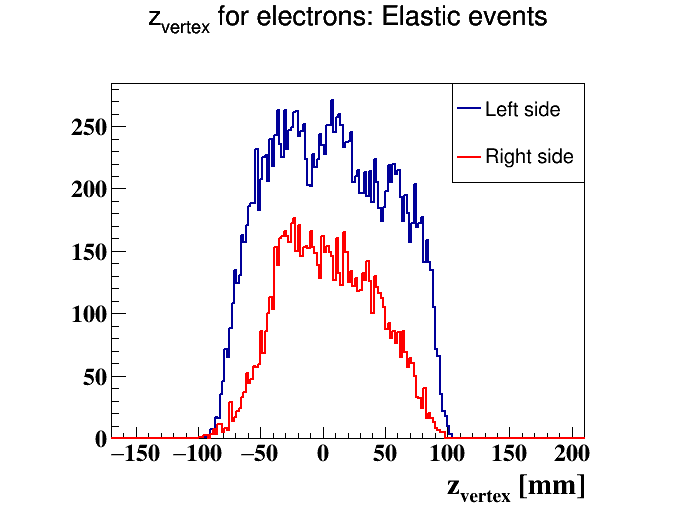
\includegraphics[scale=0.34]{fig_rtpc/updates/elastic_z_vertex.png}
\caption{z-vertex distributions for the electrons of the identified elastic 
events in the two modules of the RTPC.}
\label{fig:2-z-vertex}
\end{figure} 

In figure \ref{fig:2-r0}, we show the distribution of the radius of curvature 
for the identified elastic tracks in the RTPC. One sees that applying the other 
good track and elastic conditions eliminate all the negative tracks as well as
the tracks with $r_{0}$ less than 30 mm.
\begin{figure}[tp]
   \centering
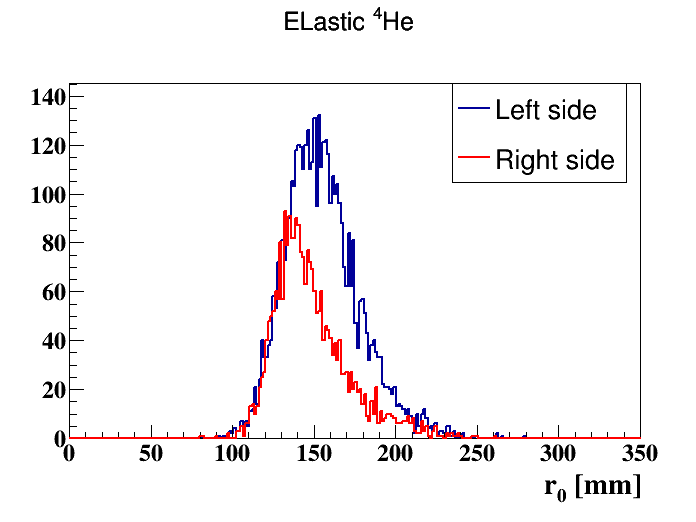
\includegraphics[scale=0.34]{fig_rtpc/updates/r0_elastic_1p2GeV.png}
\caption{The radius of curvature distributions of the identified elastic 
$^{4}$He tracks in the two modules of the RTPC after applying the other good 
track and elastic events}.
\label{fig:2-r0}
\end{figure} 

The distributions of $sdist$ and $edist$ for the identified elastic $^4$He 
elastic tracks, figure \ref{fig:2-sdist-edist}, show that the tails, 
which are mostly due to electronic noise, are removed. Therefore, making 
tighter cuts would not cause significant changes in the calibration as the 
tail regions are cleaned by the other good track and elastic cuts.

\begin{figure}[tp]
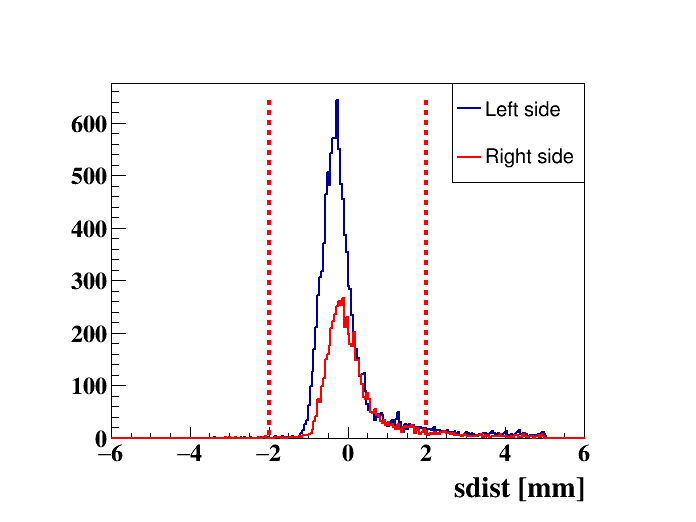
\includegraphics[scale=0.34]{fig_rtpc/updates/sdist_elastic_1p2GeV.png}
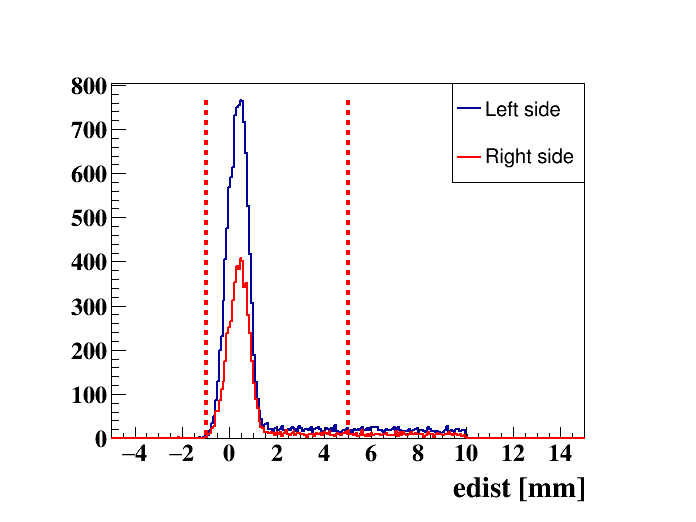
\includegraphics[scale=0.34]{fig_rtpc/updates/edist_elastic_1p2GeV.png}
\caption{ $sdist$ (on left) and $edist$ (on right) distributions for the 
identified $^4$He elastic tracks in the two modules of the RTPC after applying 
the other cuts. The vertical dashed red lines indicate the initial cuts were 
applied to select the good tracks.}
\label{fig:2-sdist-edist}
\end{figure} 



\subsection{Drift paths and drift speed calibration}

\subsubsection{Drift speed parametrization}
The electrons follow their drift paths with a certain speed, named drift 
speed. This speed is affected by the experimental conditions, such as the 
variations in the magnetic field or in the gas composition. We can measure this 
speed using the tracks detected in the RTPC, as it is explained in this 
section.


In our TPC, the electrons released close to the cathode take the maximum drift 
time ($TDC_{max}$) to reach the readout pads while the geometrical symmetry 
along the RTPC ensures that these electrons always travel the same distance.  
Therefore, by identifying the $TDC_{max}$, the drift speed can be deduced.  
Figure \ref{fig:TDC_profile} shows the time profile of the collected hits for 
the detected good tracks. The experimental drift time ranges between the 
trigger time (TDC$_{min}$ = 15 TDCs) to 75 TDCs. The time profile shows an 
expected dropping edge at high TDCs due to the geometrical constraints. In 
order to avoid the statistical effects in determining the  $TDC_{max}$, we 
define a value named as $TDC_{max/2}$ at which the dropping edge passes to half 
of the maximum number of hits in each hits-time profile. $TDC_{max/2}$ is 
inversely proportional to the drift speed.
 

We measure the $TDC_{max/2}$ along the length of the RTPC to take into account 
the variations in the electric and magnetic fields. The results can be seen in 
figure \ref{fig:RunNumber_61551_TDCmax_Zslice}, where a clear variation of the 
drift speed along the RTPC was observed.  

\begin{figure}[tbp]
\centering
\vspace{-0.1in}
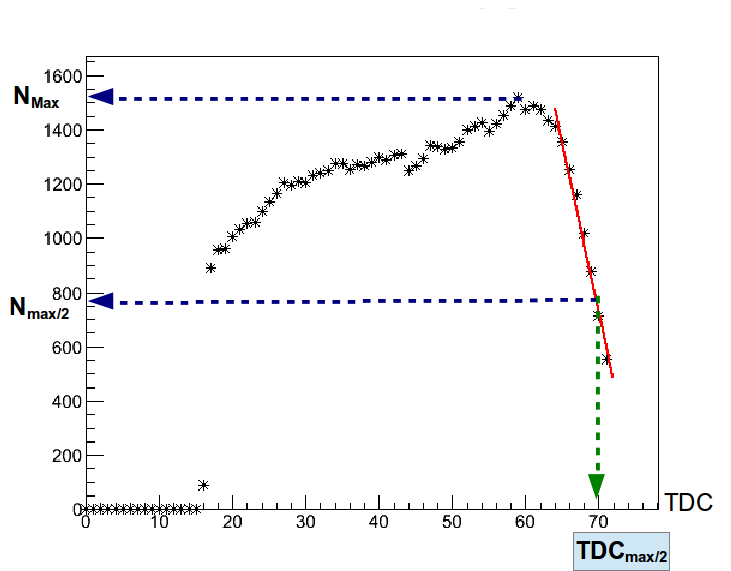
\includegraphics[scale=0.35]{fig_rtpc/TDC_profile.png}
\caption{Time profile of the collected hits for the RTPC good tracks in one 
   experimental run, run 61511, integrated over the full longitudinal length 
(z) of the RTPC. The $TDC_{max/2}$ is the time at which the dropping edge 
passes half the maximum number of hits.}
\label{fig:TDC_profile}
\end{figure} 

We also monitor the $TDC_{max/2}$ evolution during the time of the experiment, 
to take into account variations. The EG6 experiment has recorded data with 
different electron-beam energies: 1.204, 5.7, 6.064 and 1.269 GeV. The 5.7 and 
6.064 data sets have low elastic cross sections compared to the 1.206 and 1.269 
data sets. For this reason, we use all the RTPC good tracks and not only the 
elastic ones for these. Before checking the stability of $TDC_{max/2}$ over the 
experimental running period, we want to check the feasibility of using all good 
tracks for the purpose of parametrizing the drift speed. In this check, the 
$TDC_{max/2}$ identified using the good tracks of the 1.206-GeV data set is 
compared to the one identified from the elastic events of the same data sets.  
The result is shown in figure \ref{fig:TDCmax_ratio}, in which the ratio 
between the two $TDC_{max/2}$ is plotted as a function of the longitudinal 
position along the RTPC. This ratio is consistent with 1, within 1$\%$. Thus we 
can conclude that using the hits of the collected good tracks is a good 
approximation. 

\begin{figure}[tpb]
\begin{minipage}[c]{.46\linewidth}
\hspace*{-0.3in}
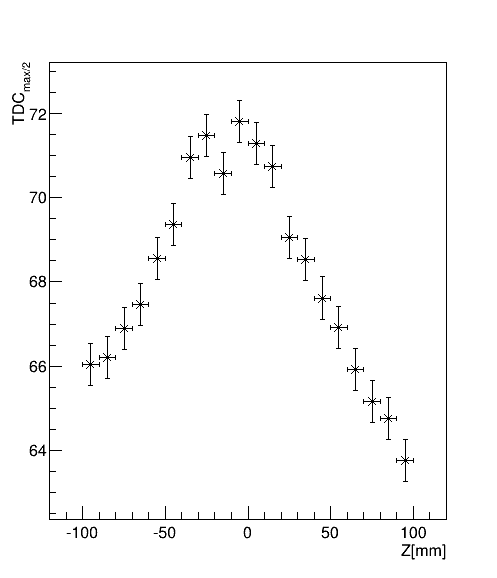
\includegraphics[height=9.5cm]{fig_rtpc/RunNumber_61551_TDCmax_Zslice.png}
 \caption{$TDC_{max/2}$ variation as a function of the longitudinal position 
 along the RTPC, $z$ position of the hit, in one experimental run, 61510.} 
 \label{fig:RunNumber_61551_TDCmax_Zslice}
\end{minipage} \hfill
\begin{minipage}[c]{.46\linewidth}
\hspace*{-0.3in}
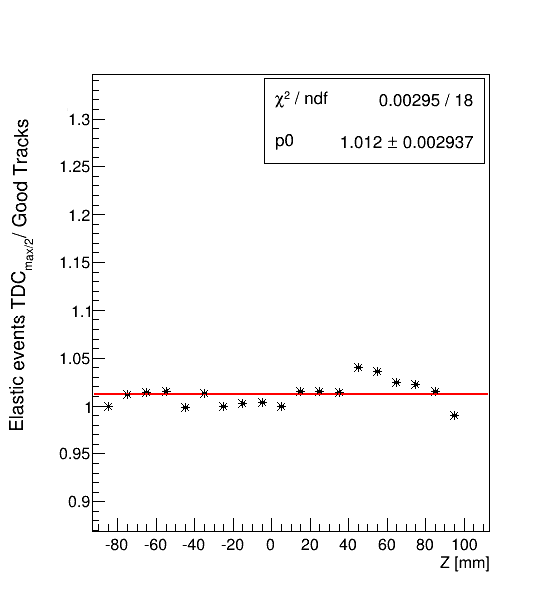
\includegraphics[height=9.0cm]{fig_rtpc/TDCmax_ratio_final.png}
\caption{Ratio between $TDC_{max/2}$ extracted using the RTPC good tracks and 
the one extracted using the clean elastic events, both from the 1.204-GeV 
dataset, as function of the hit position ($z$).}
\label{fig:TDCmax_ratio}
\end{minipage}
\end{figure}

The variations with time of $TDC_{max/2}$ are shown in figure 
\ref{fig:Drift_run_number}, in which each point is a run of about two hours of 
data taking. One can see a non-negligible variation over the three months of 
data taking due to the changes in the experimental conditions. The main cause 
of these variations is probably the variation of proportions in the drift gas 
mixture which was not perfectly under control due to leaks in the parts of 
the detector where the gas is contained by very thin aluminized mylar.

As $TDC_{max/2} -15 $ ($= \frac{Drift~path~length}{Drift~speed}$) varies with 
both run number (time) and the geometry of the RTPC ($z$ along the RTPC). We
parametrize the dependence on $z$, hit (pad) position, for each run in the 
form:
\begin{equation}
TDC_{max/2} (z)= p_{0} +  p_{1} * e^{p_{2}*(z-p_{3})^{2}}.
\label{equ:drift_speed_fit}
\end{equation}
Then fits are performed for these parameters as functions of the run number, 
such that the drift speed parametrization depends on the run and $z$ along the 
RTPC. The numeric parametrizations of $p_{0}$, $p_{1}$, $p_{2}$, and $p_{3}$ 
can be found in Appendix \ref{app:RTPC_appendix}, table \ref{Table:TDCmax}. 

The implementation of these parametrizations of the drift speed in our 
reconstruction codes resulted in more good tracks and elastic 
events identified comparing to the previous calibration sets. Figure 
\ref{fig:Drift_run_number} also shows these gain percentages of good tracks 
(GT) and elastic events (El) for a few runs. The gradual improvement 
with time is due to the improvement on the parameters of the reconstructed 
tracks ($sdist$, $edist$ ... etc), which are then more likely to pass the 
selection requirements. 

\begin{figure}[tpb]
\hspace{-0.3in}
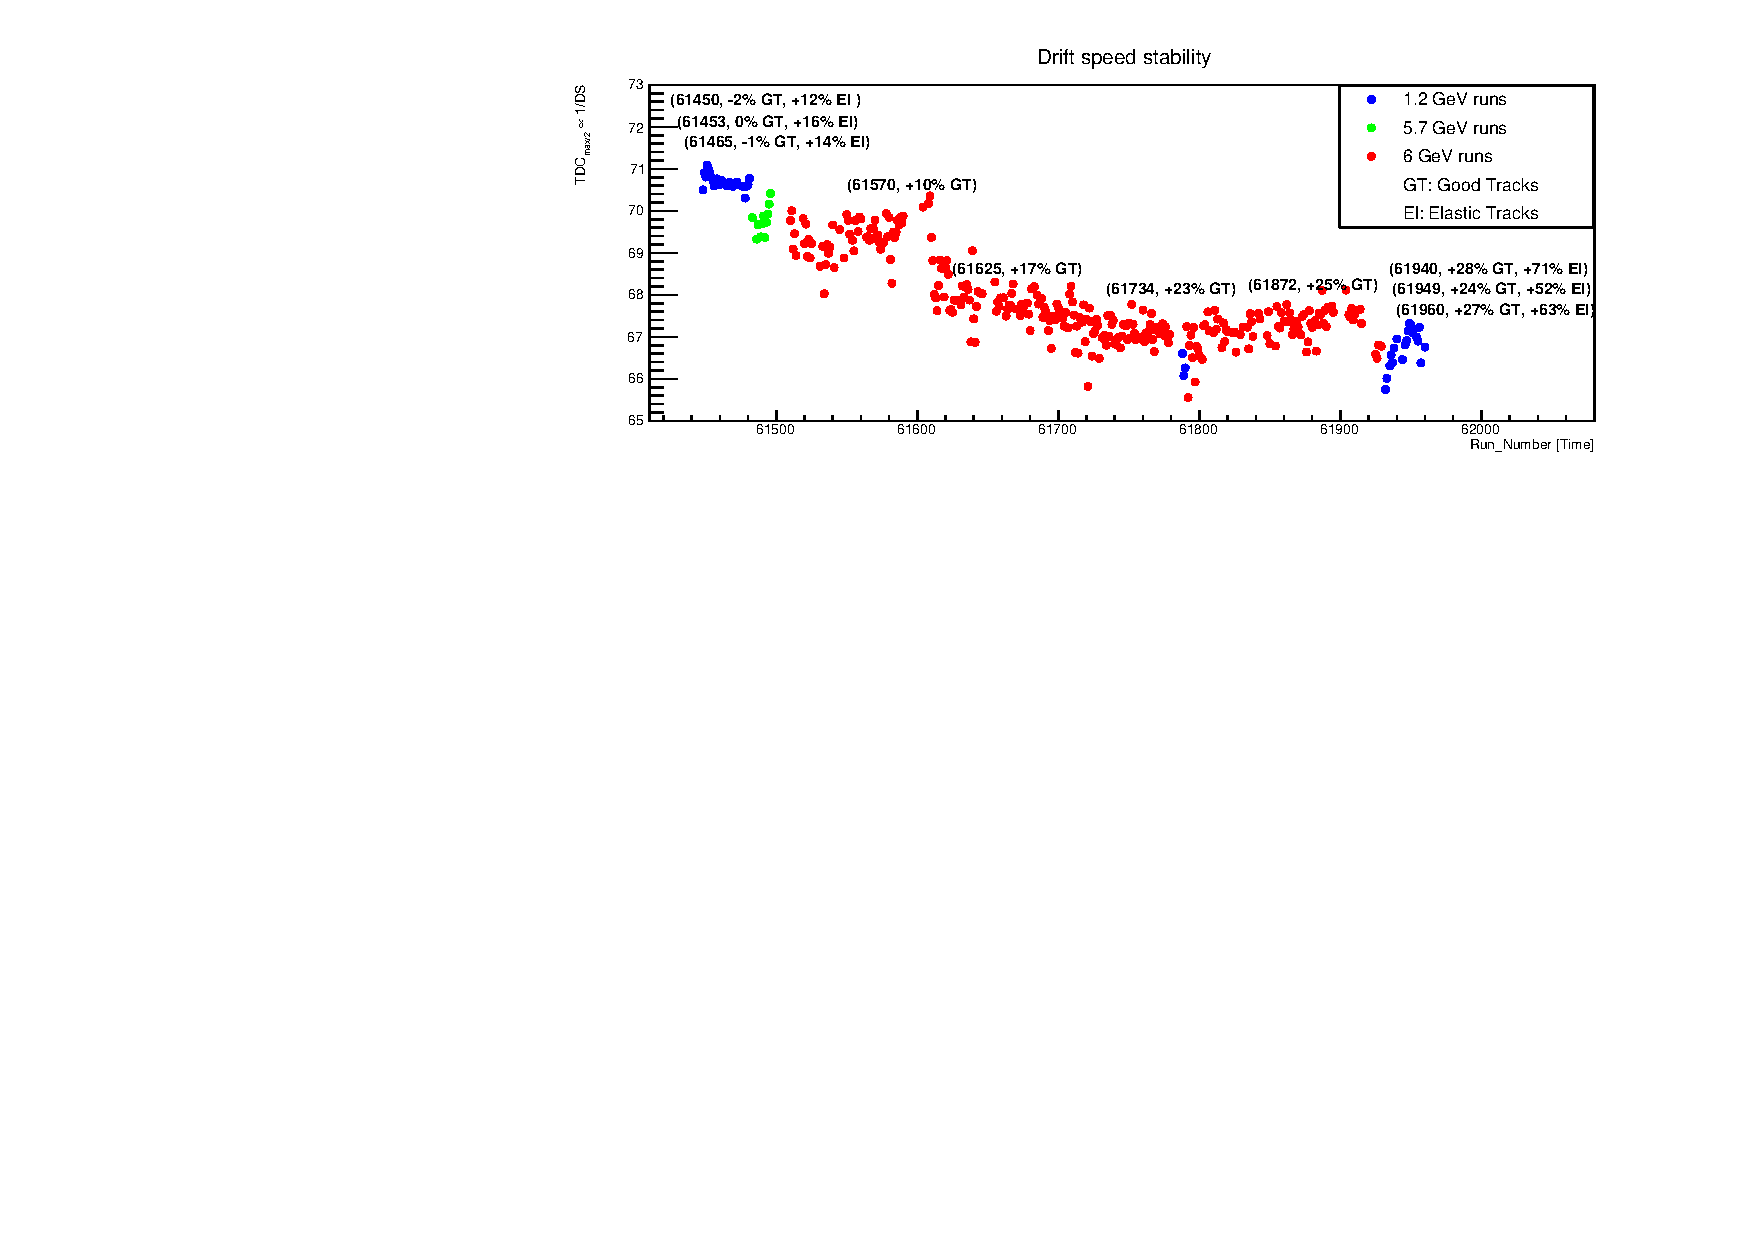
\includegraphics[scale=0.9]{fig_rtpc/updates/TDCmax2-run-number.pdf}
\caption{ The integrated $TDC_{max/2}$ over the full z-RTPC as a function of 
run number.  The gain after calibration in the collected good tracks (GT) and 
elastic events (El) are shown for a sample of runs.}
\label{fig:Drift_run_number}
\end{figure} 

\subsubsection{Drift paths parametrization}

A drift path is the trajectory that an electron follows after being 
released in the drift region. The standard software to calculate these paths is 
the MAGBOLTZ program \cite{MAGBOLTZ}. This program requires precise knowledge 
of the experimental conditions, such as the detector's geometry, the exact 
composition of the drift gas and the applied electric and magnetic fields. Thus 
any variation in these conditions would give inaccurate calculated drift paths.  
In the EG6 experiment, MAGBOLTZ has been used to calculate a first set of drift 
paths, but it was found rapidly that our lack of knowledge on some of the RTPC's 
conditions was limiting the precision of the calculation. For this reason, we 
chose to further calibrate the drift paths with a method 
that does not require an exact knowledge of the conditions in the chamber 
and is instead based on the experimental data.  

In this alternative method, we use the identified elastic ($e ~ ^{4}He 
\rightarrow e ~ ^{4}He$) events to extract the drift paths. For these events, 
the kinematic of the recoil $^{4}He$ is calculated from the scattered 
electron. Then the electrons' drift paths is extracted by comparing event
by event the experimentally measured hits in the RTPC to the 
trajectory of the corresponding simulated $^{4}He$. With this technique, the 
drift paths are obtained with limited impact from our knowledge of the 
conditions in the RTPC, in particular the method is completely independent 
from both electric field and gas mixture. 

We perform the drift paths' extraction in two passes. 
In the first pass, we assume a linear correlation between the 
radius of emission $R$ (we work here in radial coordinates: $R$ and $\phi$) and the 
drift time to link GEANT4 hits along the trajectory to actually measured 
hits. Based on this association, we obtain a $\Delta \phi$ distribution 
as function of time. $\Delta \phi$ is the 
difference between the $\phi$ observed in GEANT4 and the $\phi$ of the pad 
which actually measured a correlated hit. Assuming we have an axial 
symmetry of the drift path, $\Delta \phi$ as a function of time indicates 
how much the electron drifted because of the magnetic field for any hit. 
This is therefore the relevant information to reconstruct the origin
of the hits measured in the detector.
However, the actual correlation between time and radius is not exactly
linear. So we perform a second pass, in which we refine the initial 
correlation between the radius and the time using the drift paths obtained 
in the first path. We then repeat the procedure of the first pass to extract 
the final drift paths. Because of the variations in the magnetic 
field along the detector, the extraction is made in $z$ bins. 

The detailed steps of the procedure are as follow:
\begin{itemize}
\item We first select a sample of well identified elastic events in our 
   experimental data. Using the
   kinematics of the scattered electrons in these events, we generate in GEANT4
   a sample of events identical to the measured ones. 
\item  For each couple of events (the experimental one and its simulated equivalent)
   we make a linear correlation between $R$, from simulation, and TDC from 
   real data, to link the GEANT4 hits to the measured ones. In our TPC, the 
   maximum $R$ equals 60 mm (close to the anode) at the trigger time, 
   (TDC$_{min}$ = 15 TDCs), and the minimum $R$ equals 30 mm (close to the 
   cathode) at maximum TDC ($TDC_{max}$). Thus, the linear correlations can be 
   written as:
\begin{equation}
   R(TDC) = \frac{60-30}{15-TDC_{max}} (TDC-15) + 60.
\label{equ:R_TDC}
\end{equation}
We apply 3 TDCs-wide windows around the linear R-TDC correlation to associate 
the GEANT4 simulated hits to measured hits. Figure \ref{fig:R_correlation} 
shows the distribution of $R$ versus TDC for to select the matched hits.
\item From these selected matched hits, we obtain $\Delta \phi$ (= 
   $\phi_{sim.}$ - $\phi_{hit\_pad}$) as a function of time. The results can be seen in 
   figure \ref{fig:1st_pass_delta_phi}\footnote{$\Delta \phi$ at the anode (TDC = 15) 
   is not equal to zero because there is a drift in $\phi$ between the anode 
   (the first GEM layer at radial distance equal to 60 mm) and the readout pads 
   (at radial distance equal to 69mm).}. This figure is fitted to obtain the 
   parameterization of the drift path.
\begin{figure}[tpb]
\centering
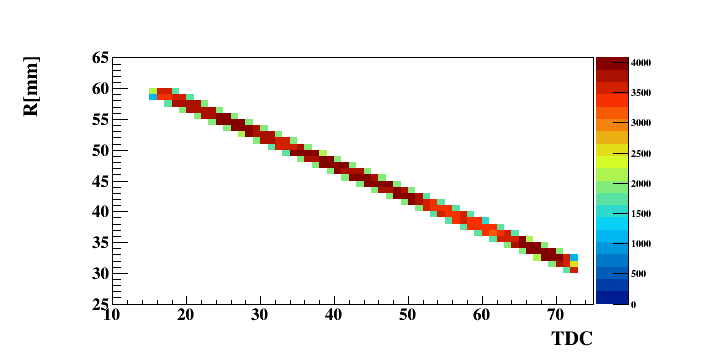
\includegraphics[scale=0.45]{fig_rtpc/updates/TdcR_check_p1_10.png}
\caption{(First pass). Distribution of $R$ as a function of time (in TDC) for the 
simulated hits located in one $z$ bin. The width of the bin is 10 mm, with the 
center at $z$ = 5 mm.}
\label{fig:R_correlation}
\end{figure}
\begin{figure}[tpb]
\centering
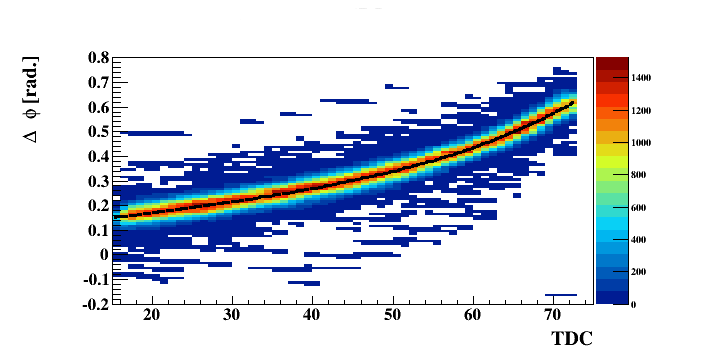
\includegraphics[scale=0.45]{fig_rtpc/TdcPhi_p1_10.png}
\caption{(First pass). Distribution of $\Delta \phi$ as a function of time (in TDC) for 
   in one $z$ bin. The width of the bin is 10 mm, 
with the center at $z$ = 5 mm. The black line represents a fit for 
$\Delta\phi$.  }
\label{fig:1st_pass_delta_phi}
\end{figure} 
\begin{figure}[tbp]
\centering
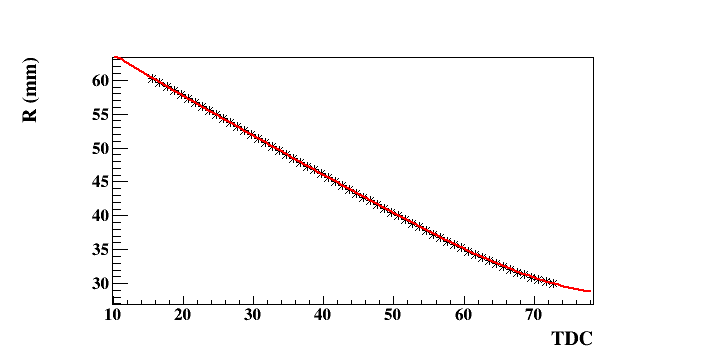
\includegraphics[scale=0.45]{fig_rtpc/TdcR_p2_10.png}
\caption{(Second pass). The calculated $R$ as a function of time (in TDC) is corrected by 
the $\Delta \phi$ relation extracted from the first pass.}
\label{fig:R_TDC}
\end{figure}
\item The correlation between $R$ and the time is then refined using the extracted  
   $\Delta \phi$ as a function of time as:
\begin{equation}
   R (TDC) = R_{min} + \bigg[\sum\limits_{i=TDC_{Max}}^{TDC} \sqrt{DS^{2} - 
      R^{2}(i) \cdot \left(\frac{\partial \Delta \phi}{\partial TDC}(i) 
\right)^{2}}~~~~\bigg] \cdot TDC,
 \end{equation}
where DS is the average drift speed, equal to 0.7 mm/TDC ( 6.14 $\mu$m/ns), 
$R_{min}$ equals to 30 mm, $R(i)$ is the linear correlation defined in equation 
\ref{equ:R_TDC} and $\Delta \phi (i)$ is the fit in figure 
\ref{fig:1st_pass_delta_phi}. The sum is multiplied by a TDC unit (=114 ns).  
The calculated R, figure \ref{fig:R_TDC}, is almost linear, 
indicating that only two itterations are probably enough.
\item In the second pass, we use the newly found $R$(TDC) relation to construct 
new $\Delta \phi$ distributions, see figure \ref{fig:final_drift_paths} for our final
result.
\begin{figure}[tp]
\centering
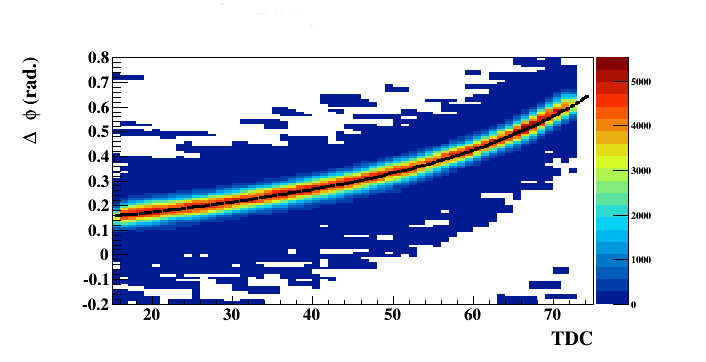
\includegraphics[scale=0.45]{fig_rtpc/FitResult_p2_10.png}
\caption{(Second pass). Distribution of $\Delta \phi$ as a function of time (in TDC) 
located in the same $z$ bin shown in figure \ref{fig:1st_pass_delta_phi}. The 
black line represents the final drift paths.}
\label{fig:final_drift_paths}
\end{figure}
\end{itemize}

We performed a third pass in which the $R$(TDC) correlation is refined using the 
drift paths from the second pass. As a 
result, we observed no difference between the drift paths of the second and the 
third passes. In other words, extracting the drift paths from two iterations 
gives us stable results. 
 
The first drift paths were extracted using the elastic events from the early 
1.204~GeV dataset. In order to ensure the consistency of these drift paths over 
the experimental running period, we extracted another set of drift paths using 
the elastic events of the 1.269 GeV dataset. We observed no difference between the 
two sets of the drift paths, ensuring the stability over the experimental 
period. The final drift paths are 
extracted using both datasets, 1.204 and 1.269 GeV. They take the form:
\vspace{-0.1in}
\begin{equation}
\Delta \phi (TDC, z)=  \sum\limits_{i=0}^{4} p_{i}(z)*TDC^{i},
\end{equation}
where the parameters, $p_{0}$, $p_{1}$, $p_{2}$, $p_{3}$ and $p_{4}$ are 
functions of $z$, as can be seen in Appendix \ref{app:RTPC_appendix}, table 
\ref{table:drift_paths}. The final drift paths are implemented in our 
reconstruction codes such that the reconstructed position of each hit becomes:
\begin{equation}
\phi_{exp}(z, TDC) = \phi _{hit\_pad} - \Delta \phi (z, TDC).
\end{equation} 

It is important to note that the drift paths have shown strong sensitivity 
to the other RTPC calibrations. Therefore, we performed iterative extractions 
of the drift paths and, as a results, obtained more good tracks with a signal 
to background ratio largely improved. Figure \ref{fig:sdist_comp_pass1v1_v6} 
shows an illustration of the improvements in terms of the $sdist$ parameter 
using the same initial collected data with an old drift paths and a newer set.

\begin{figure}[tp]
\centering
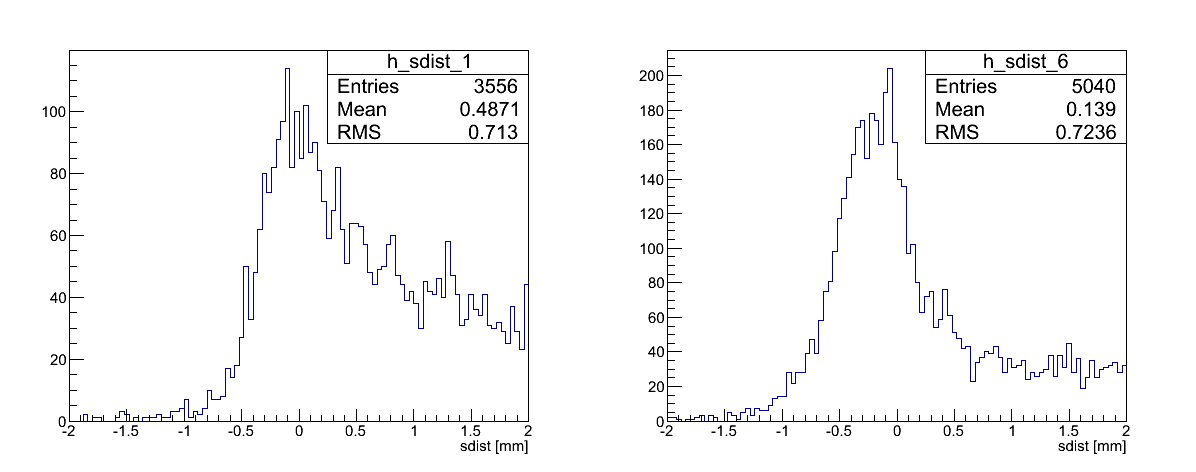
\includegraphics[scale=0.38]{fig_rtpc/sdist_comp_pass1_v1_v6.png}
\caption{The $sdist$ distribution for the collected tracks in the RTPC using 
the same initial collected data with an old set of drift paths, on the left, 
and a newer set, on the right.}
\label{fig:sdist_comp_pass1v1_v6}
\end{figure}

\subsubsection{Summary}
The drift paths and drift speed were first extracted using the
MAGBOLTZ Monte Carlo simulation. One can find the detailed procedure of
a similar extraction in the BoNuS analysis note \cite{GEM_holes}.
Then, we improved this first result with many iterations after each change that 
would affect the drift paths, such as the beam-offset and gain calibrations of 
the RTPC. Moreover after each pass, the number of elastic events used for 
calibration increased, justifying by itself a new calibration. Overall, this 
was a long process that evolved and improved over the years and we concentrated 
in the note on the description of the final iteration of this calibration.


\subsection{Gain calibration}
The second important calibration is the amplitude of the signal provided in ADC 
units. Since each charged particle deposits a certain amount of energy 
($\small{\frac{dE}{dX}}$) when crossing a material, we can identify particles 
based on this variable. The ($\small{\frac{dE}{dX}}$) depends on the 
characteristics of the particle, such as its energy, mass and charge, and the 
nature of the medium as well. 

$\small{\frac{dE}{dX}}$ can be calculated using the Bethe-Bloch formula \cite{bethe_block}:
\begin{eqnarray}
\left\langle \frac{dE}{dX} \right\rangle &=& \rho K z^{2} \frac{Z}{A} 
   \frac{1}{\beta^{2}} \left[ \frac{1}{2} ln 
   \left(\frac{2m_{e}c^{2}\beta^{2}\gamma^{2}T_{max}}{I_{max}} \right) - 
\beta^{2} -\frac{\delta\beta\gamma}{2}\right]\\
\text{with }
T_{max} &=& \frac{2m_{e}c^{2}\beta^{2}\gamma^{2}}{1+2\gamma m_{e}/M + (m_{e}/M)^{2}} 
\end{eqnarray}
where $T_{max}$ is the maximum kinetic energy of a free electron in a single 
collision, and $z$, $M$, $\beta$ are the charge, mass and speed (=$p/ \sqrt{M^2 
+ p^2}$, where $p$ is the momentum) of the particle, respectively.  $m_{e}$ is 
the electron mass and the constant $K$ is equal to $4 \pi N_{A} 
r^{2}_{e}m_{e}c^{2}$ = 0.307075 MeV mol$^{-1}$ cm$^{2}$. $Z$, $A$, $I$, $\rho$ 
are the effective charge, atomic number, mean excitation energy and mass 
density of the medium. In the RTPC, these constants are equal to 66, 126.79 mg 
mol$^{-1}$, 99.79 eV and 1.03 mg/cm$^3$, respectively. 

Experimentally, $\small{\frac{dE}{dX}}$ can be calculated from the collected ADCs as: 
\begin{equation}
 \left\langle \frac{dE}{dX} \right\rangle= \frac{\sum\limits_{i} \frac{ADC_{i}}{Gi}}{vtl},
\end{equation}
where the sum runs over all the pads contributing to a track. $ADC_{i}$ is the 
recorded amplitude in each pad $i$, and $G_{i}$ is its gain. The $vtl$ is the 
total visible length of the track in the active drift volume. This is of course 
assuming the energy loss in the drift region is small in regard to the total 
energy of the particle, which is true except close to our detection 
threshold.

The electron collection system of the RTPC has 3200 readout pads. The gain of 
each pad is the ratio between the deposited energy and the output recorded 
value. We extracted the gains using two techniques. The first one is by 
comparing the experimental recorded $\small{\frac{dE}{dX}}$ to the expected 
values calculated from the Bethe-Bloch formula. The second technique is based 
on comparing the experimental ADCs to the GEANT4 simulated ones, track by 
track. We latter refined this second method by comparing the ADCs of each pad 
to the average ADCs of the other pads in the same track.

The two techniques were investigated for the EG6 experiment using the elastic 
events from the 1.206 GeV data set. The first method involves a series of 
equations to be solved to obtain the gains.
 
The second method requires improvements in the simulation, in order to 
match the real experiment. In summary, these improvements are:
\begin{itemize}
\item Implementation in the simulation of the previously extracted 
   parametrizations of the drift speed and the drift paths.
\item Global ADC normalization to give reasonable simulated values. In the left 
   module, 1 ADC is equal to 17 eV, while it is equal to 21 eV in the right 
   module. These normalizations were extracted from the comparison of the data 
   to the GEANT4 simulation.
\item Rejection of the signals from bad pads. During the experiment, the 
   readout system of the RTPC suffered from 555 dead or noisy pads. These pads 
   are marked by the dotted squares in figure \ref{fig:pad_row_col}.
\item Smearing the position of the simulated hits. Experimentally, the average 
   number of hits per track is around 80 while the initially reconstructed mean 
   value from the simulation is around 50. We apply a Gaussian smearing on the 
   position of the simulated hits to make the simulation more realistic, see 
   figure \ref{fig:NNb_hits}.  
\item Application of the TPC's DAQ cut on the simulated data. Experimentally, 
   each pad must have at least 3 consecutive time bins, with ADC values above 
   the threshold, 35 ADCs, in order to be recorded. Then, the hits of three 
   neighboring bins on each side of the above threshold bins are also recorded, 
   while the other hits are not.
\end{itemize} 

\begin{figure}[tpb]
\centering
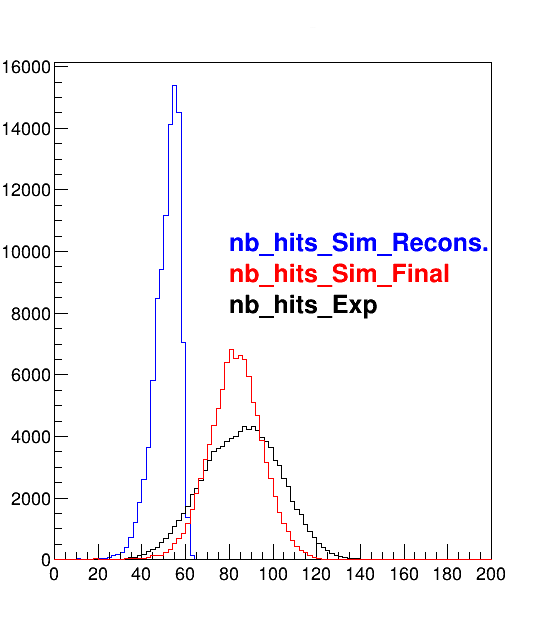
\includegraphics[scale=0.35]{fig_rtpc/NNb_hits.png}
\caption{The distributions of the number of hits per track. The black, the blue 
and the red distributions are the number of hits per track  for respectively, 
the experimental data, simulation before smearing and the simulation with 
smearing.}
\label{fig:NNb_hits}
\end{figure}

To illustrate the procedure of comparing simulated tracks with real tracks,
we show in Figure \ref{fig:EVENT_adc_tdc} the simulated and the experimental 
ADCs as a function of the TDCs for the same track. Then, the gain of each pad 
is defined as the ratio between the mean recorded experimental ADCs to the mean 
simulated ADCs in the same track. Then for each pad, the gain ratios were 
collected from all the identified elastic tracks and these gains were fitted by 
a Landau function to give a first pass gain for each pad as the most probable 
value of the fit. 

\begin{figure}[tpb]
\centering
\vspace{-0.1in}
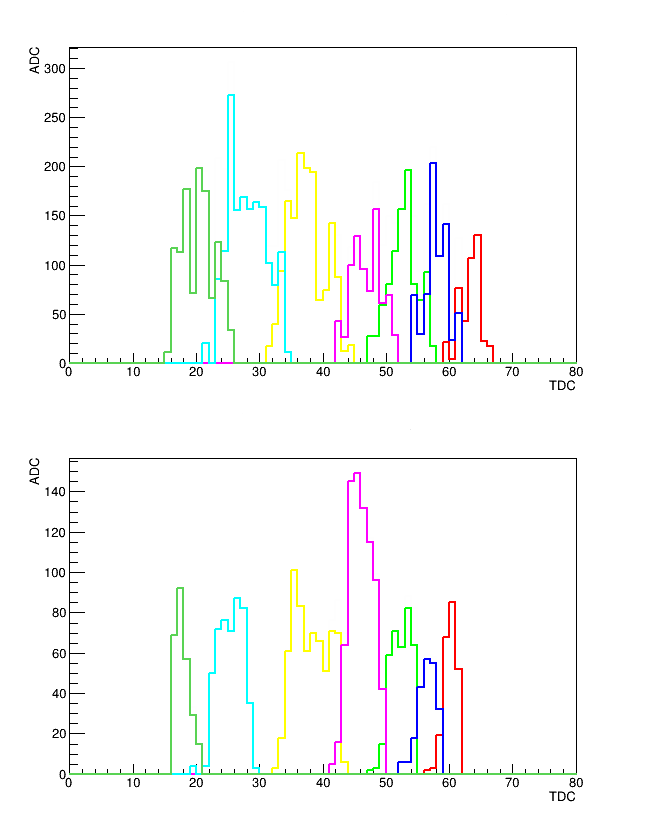
\includegraphics[scale=0.320]{fig_rtpc/EVENT_adc_tdc.png}
\caption{The simulated (top) and the experimental (bottom) ADCs versus TDC 
distributions for the same track. The same colors indicate hits that were 
registered in the same channel for the simulation and the experiment.}
\label{fig:EVENT_adc_tdc}
\end{figure}

To make sure that the recorded ADCs by a given pad are similar to the recorded 
ADCs by other pads in the same track, we refined this calibration after the 
extracted gains were applied to the experimental data. At this step, we 
compared the mean ADCs of each pad to the mean ADCs of the whole track. This 
ratio is collected from all the elastic events and a gain correction factor is 
extracted and applied to get a final gain for each pad, labeled as second pass 
gain in figure \ref{fig:dedxre}. 


As the two modules of the RTPC are electronically separated, we look at their 
calibrations separately. Figure \ref{fig:dedxre} shows the ratio between the 
calculated $\small{\frac{dE}{dX}}$, using the gains extracted from first and 
the second (both passes) meothods, and the GEANT4 simulated 
$\small{\frac{dE}{dX}}$ for the elastic events in the two modules of the RTPC.  
From the latter figure, one can see improvments obtained by using this method 
to fine tune the gains extracted only by comparing data to simulation. We 
conclude that extracting the gains from comparing data to simulation in terms 
of the ADCs of the individual tracks gives more precise gains than solving the 
series of equations. Figure \ref{fig:pad_row_col} shows the gains from the 
second method, where the dotted squares refer to the dead or noisy pads. These 
are the ones that are implemented in the EG6 reconstruction codes.


\begin{figure}[tpb]
\hspace{-0.5 cm}
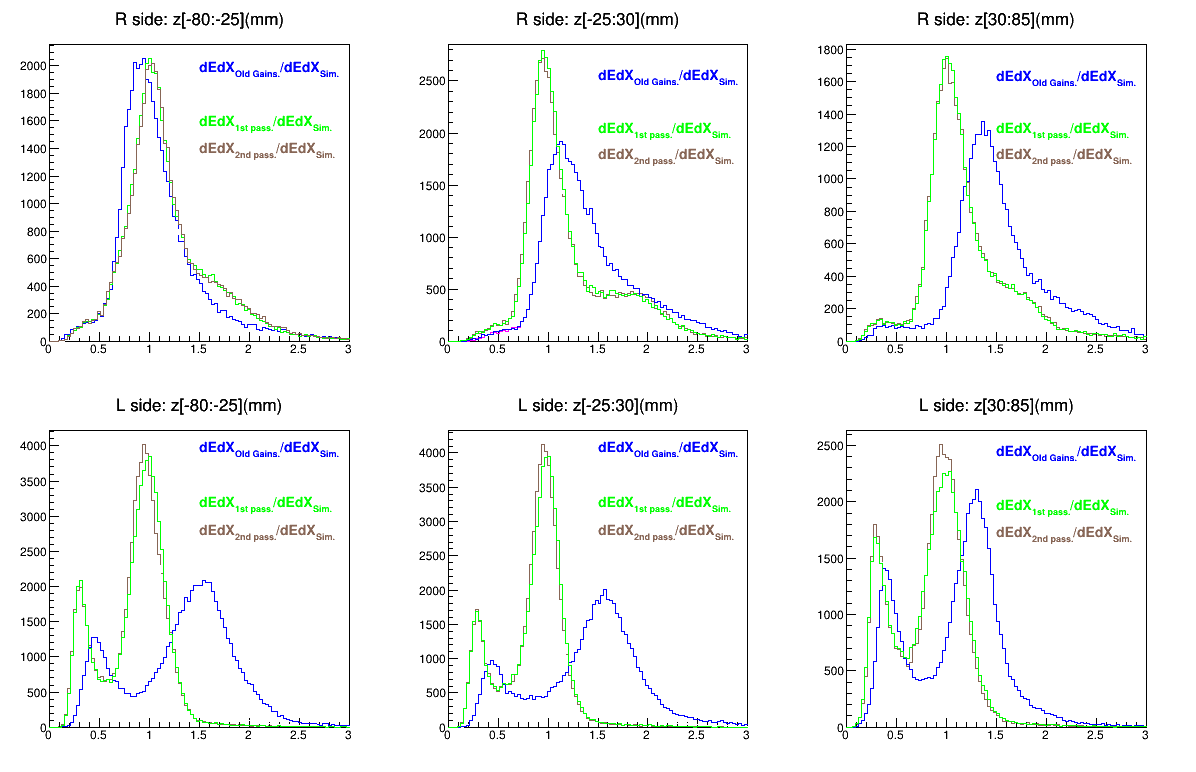
\includegraphics[height=11.5cm]{fig_rtpc/updates/dedx_ratio_elastic_NAB.png}
\caption{The ratio between the experimental dEdx and the simulated ones for 
   different regions along $z$ for the two modules of the RTPC, right module on 
   top panel and left module on bottom panel. The blue lines are using the 
   first method of extracting the gains (comparing the experimental recorded 
   dEdx to the expected values calculated from the Bethe-Block formula). The 
green lines are using the fist pass of the second method (comparing simulation 
to data only) with all the elastic event sample. The brown lines are using the 
final gains extracted from the second method (both passes).}
\label{fig:dedxre}
\end{figure}


%\begin{figure}[tbp]
%\centering
%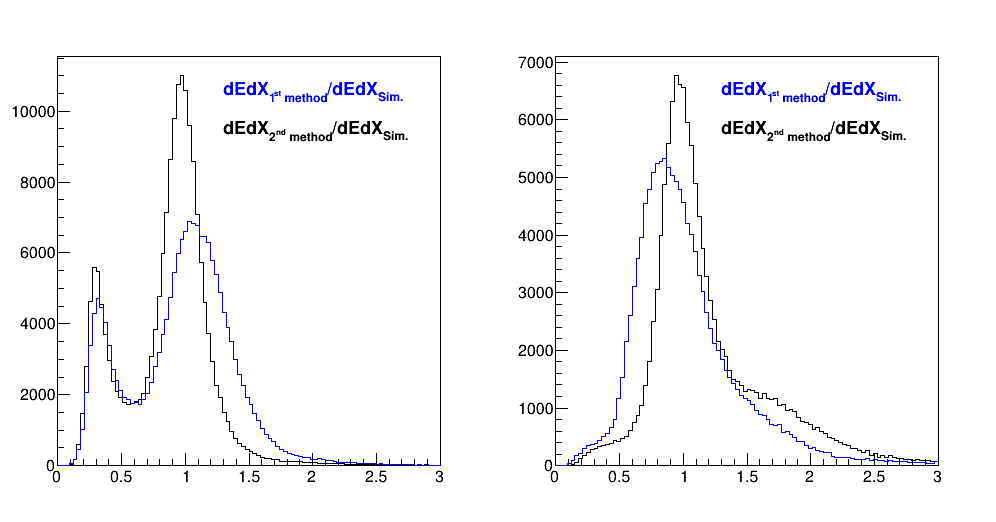
\includegraphics[scale=0.400]{fig_rtpc/dedx_p_sim_exp_2nd.png}
%\caption{The ratio between the experimental $dE/dx$, using the gains obtained 
%with the two methods (1$^{st}$ in blue, and 2$^{nd}$ in black), to the GEANT4 
%simulated $dE/dx$, plotted for the two modules of the RTPC, respectively left 
%nd right. }
%\label{fig:dedx_p_exp_2nd}
%\end{figure}

\begin{figure}[tbp]
\centering
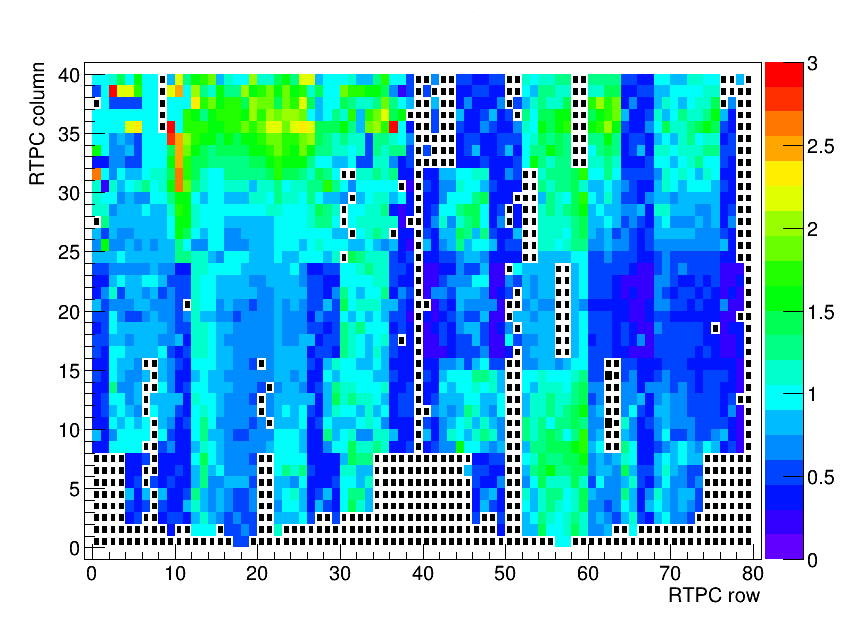
\includegraphics[scale=0.300]{fig_rtpc/pad_row_col.png}
\caption{The extracted gains from the second method. The dotted squares refer 
to the position of the excluded pads.}
\label{fig:pad_row_col}
\end{figure}

In the left module of the RTPC, on the bottom panel of figure \ref{fig:dedxre}, 
one notices an additional unexpected lower peak (dEdx$_{exp}$/dEdx$_{sim} \sim$ 
0.3). These events pass all the elastic requirements but for some reasons they 
have lower ADC values. They represent around $7\%$ of all the elastic events.  
After extended studies, the nature of these particles is not identified yet. We 
note that this is a global phenomenon in the left module as 94$\%$ of the left 
module's pads are involved in both some low and high dEdx events. For instance, 
figure \ref{fig:Chann_706} shows the average ADC versus TDC distributions for 
the recorded hits in one of these pads in the left module. For the calibration 
procedures, the events with low dEdx were excluded as we do not fully 
understand their nature, see figure \ref{fig:dedx_cal_left}.
\begin{figure}[tbp]
\centering
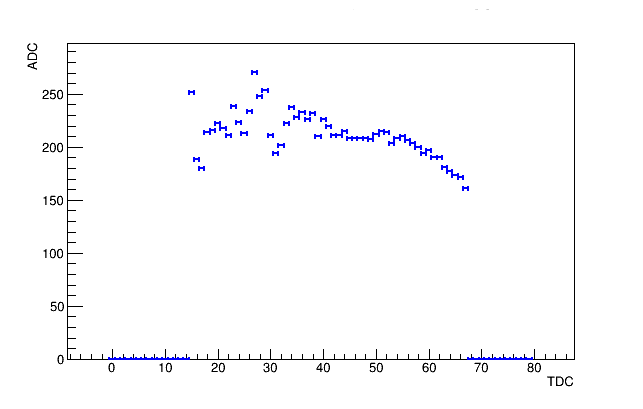
\includegraphics[scale=0.4]{fig_rtpc/Chan_706_1.png}
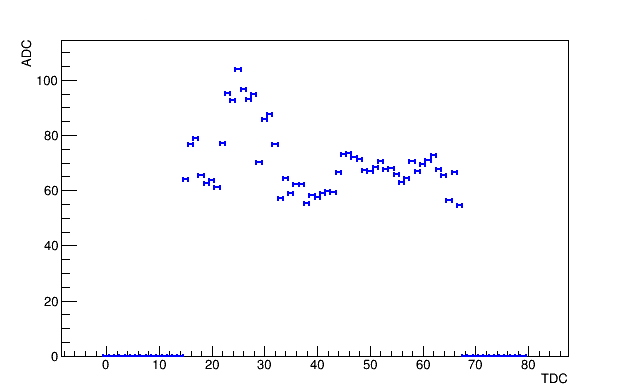
\includegraphics[scale=0.4]{fig_rtpc/Chan_706_2.png}
\caption{The average ADC vs. TDC distributions of the experimental hits 
   recorded for the elastic events in one pad of the left module, pad number 
   706.  On the top: the distribution for the elastic tracks in the region 
   where dEdx$_{exp}$/dEdx$_{sim} $ $\sim$ 1. On the bottom: the distribution 
for the elastic tracks that exhibit dEdx$_{exp}$/dEdx$_{sim} $ $\sim$ 0.3.}
\label{fig:Chann_706}
\end{figure}

\begin{figure}[tbp]
\centering
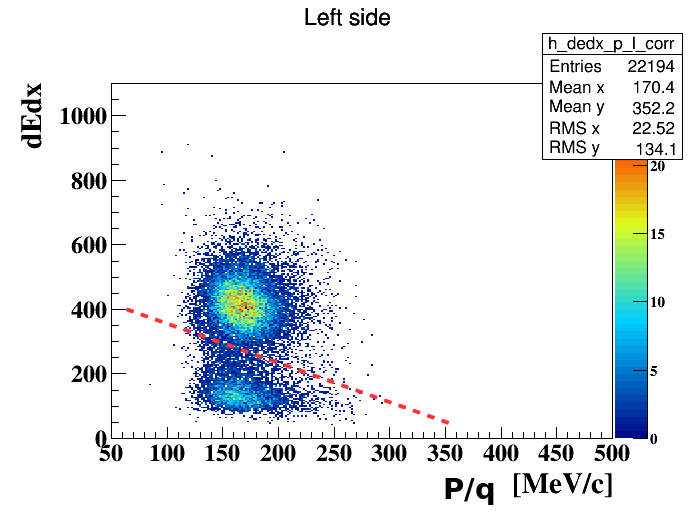
\includegraphics[scale=0.4]{fig_rtpc/dedx_l_cal_cut.png}
\caption{DEdx as a function of the measured momentum inside the left module of 
the RTPC for a sample of the identified elastic $^{4}He$ tracks. The red dashed 
line represents the cut we applied to exclude the low dEdX events from usage 
for the calibration purposes explained earlier in this chapter.}
\label{fig:dedx_cal_left}
\end{figure}




To check the validity of the extracted gains, we show $\small{\frac{dE}{dX}}$ 
versus the momentum (per charge unit) measured in the RTPC for all the 
collected tracks of the 1.206 GeV data set. In the plots, we add the 
theoretical lines derived from the Bethe-Bloch formula for possible detected 
particles: $^4He$, $^3He$, $^3H$, Deuterium (d) and the protons.
\begin{figure}[tbp]
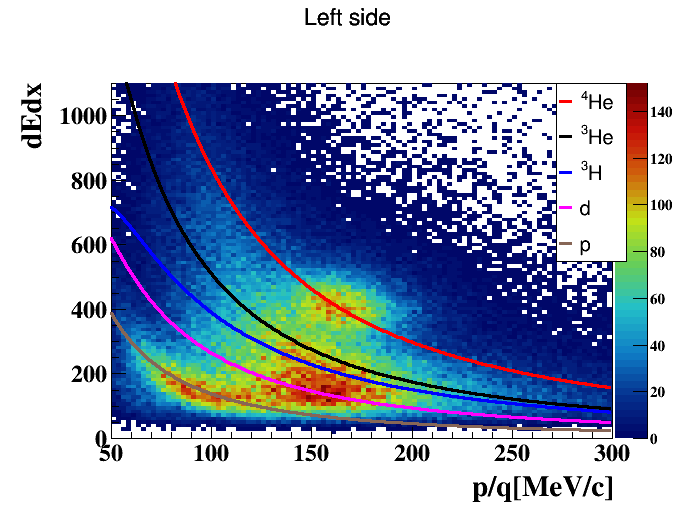
\includegraphics[scale=0.35]{fig_rtpc/updates/dedx_p_l.png}
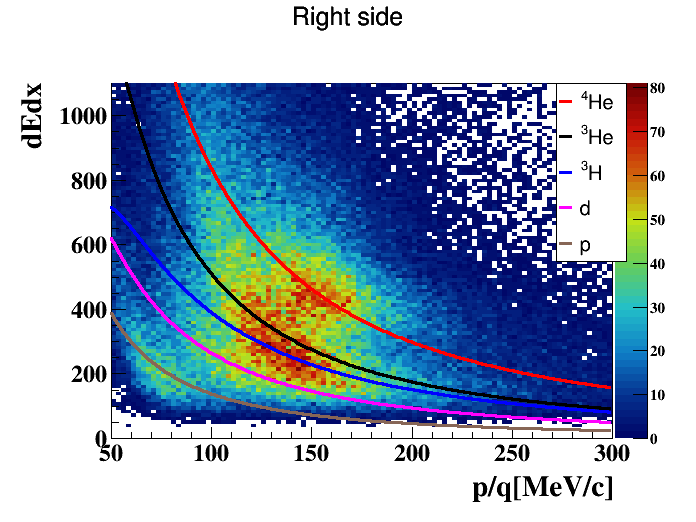
\includegraphics[scale=0.35]{fig_rtpc/updates/dedx_p_r.png}
\caption{The experimental $\small{\frac{dE}{dX}}$ calculated using the second method gains versus $p/q$ of all the collected good tracks in the RTPC in the early 1.204 GeV dataset.}
\label{fig:dedx_all}
\end{figure}
One can see the different bands corresponding to the different detected particles.  
Even though the bands are very wide, the $\small{\frac{dE}{dX}}$ can be used to 
perform particles identification for large data set and different physics 
processes. In this analysis, the $\small{\frac{dE}{dX}}$ is not used to 
identified the recoil $^{4}He$ in the coherent DVCS event selection, as the 
 set of exclusivity cuts that will be 
presented in chapter 4 appears to be strict enough.

\subsection{Noise rejection}
\label{sec:noise_rejection}
The RTPC was designed to reduce noise and contribution from M\o ller 
electrons via the first and second 1 atm gas gaps. During data taking, the 
readout thresholds of the RTPC were set low to avoid efficiency problems, with 
the effect of recording more electronic noise. The latter effect is illustrated 
by the large occupancies in the top panel of 
figure~\ref{fig:occ_noiserej}.  

Two independent noise signatures were found, and event-based algorithms were implemented to significantly reduce them offline. This resulted in improved track quality, increased track efficiency, and the opportunity to reintroduce channels otherwise determined to be too noisy.  This also resulted in more uniform occupancy, shown in the bottom panel of figure~\ref{fig:occ_noiserej}.  

Here we describe the methods and their specific effects. These are implemented 
in EG6's pass2 reconstruction in \texttt{\$CLAS\_PACK/gem/noisypads.c}.

\subsubsection{Oscillatory Noise}
An oscillatory noise signature was found for many RTPC readout pads, and is 
attributed largely to the electronics. The signature is a series of hits 
falling on a fixed ADC vs TDC curve for TDC less than 30.  About 18\% of the 
active pads have very strong contributions from this type of noise, which 
previously resulted in many of them being marked as ``bad'' due to high 
occupancies.

An algorithm was developed to remove hits corresponding to this noise without 
suppressing good hits.  First, the ADC vs TDC noise curve was parameterized.  
Next, for every event and channel independently, the number of hits falling on 
this curve is counted.  If a significant number of hits lie far above or below 
the noise curve, no rejection is performed.  If most of the hits below TDC=30 
fall on the noise curve, all hits below TDC=30 are rejected for that channel.  
Figure \ref{fig:Adcvstdcnoise} shows the effect of this noise reduction for one 
very noisy pad. The result of this algorithm is 5$\%$ more good tracks 
reconstructed, with improved signal to background ratio, as can be seen in 
figure \ref{fig:noise_edist_}.  Further, this allowed to recover 40 channels 
that had previously been ignored due to high occupancies before this noise 
rejection.

\begin{figure}[tbp]
\centering
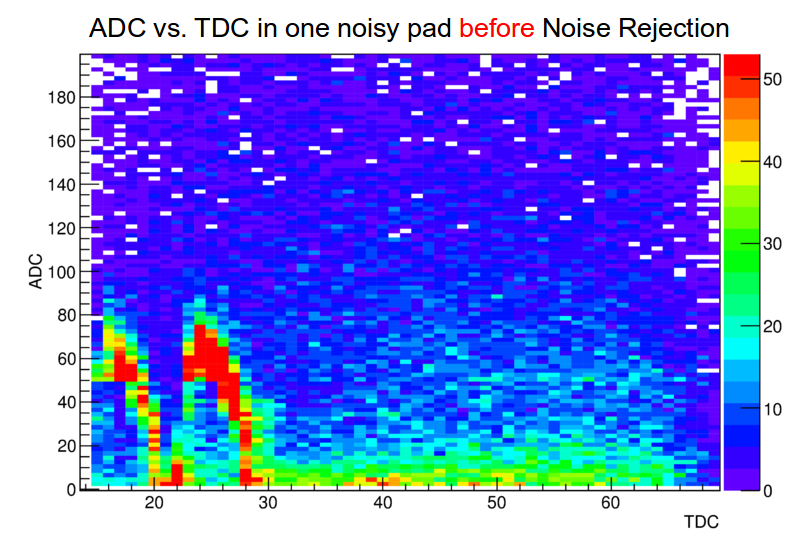
\includegraphics[scale=0.3]{fig_rtpc/noisy_pad_before_rejection.png}
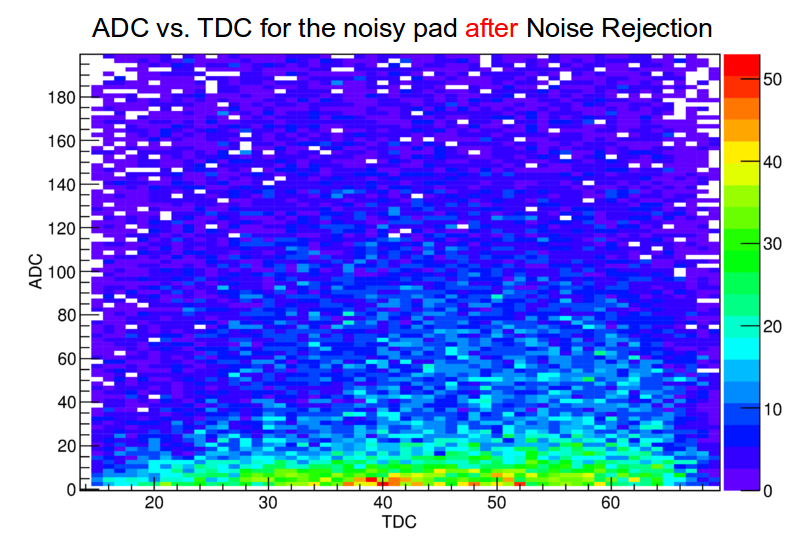
\includegraphics[scale=0.3]{fig_rtpc/noisy_pad_after_rejection.png}
\caption{The integrated ADC vs. TDC of the hits for good tracks before (left) 
and after (right) the oscillatory noise reduction, for a particular pad with 
strong noise. The color scale on the z-axis is for the hit yield and identical 
in both plots as well as the event sample.}
\label{fig:Adcvstdcnoise}
\end{figure}

\begin{figure}[tbp]
%\hspace{-0.4in}
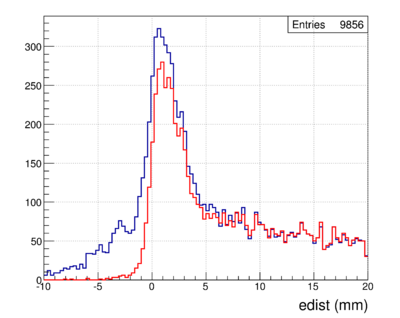
\includegraphics[scale=0.55]{fig_rtpc/400px-Edist_noiserej.png}
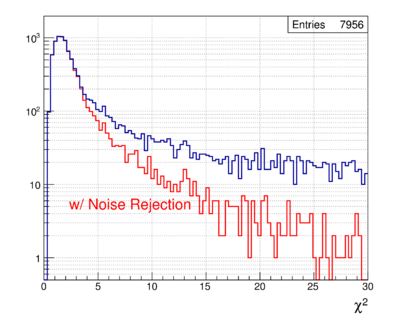
\includegraphics[scale=0.55]{fig_rtpc/400px-X2_noiserej.png}
%\vspace{-0.1in}
\caption{The $edist$ (left) and the $\chi^{2}$ (right) distributions for all 
the tracks collected in the RTPC before (blue) and after (red) the oscillatory 
noise rejection. The event sample and color scales are identical in both 
plots.}
\label{fig:noise_edist_}
\end{figure}

\subsubsection{Readout Group Noise}
Another noise signature is isolated to particular readout boards, corresponding 
to 8x2 channel groups. Initially many of these 8x2 groups were ignored in 
reconstruction due to very high occupancy (see figure \ref{fig:occ_noiserej}).  
Upon further analysis, we found many events where these groups behaved normally 
and measured good tracks, while in other events the whole 8x2 channel group 
fired. In other words, the noise level of channels within the groups is 
correlated in time.

An event-based method was implemented to treat this noise by computing an event 
pedestal for the entire group for cases when there exist neighboring hits.
Hits in the 8x2 with no neighboring hits outside the group were used to 
calculated an event pedestal for the group. That pedestal is subtracted off all 
hits in the board in that event. If there are no neighboring hits outside the 
8x2 group, the whole group is rejected in that event. 

The effect of this algorithm on a couple reconstructed tracks is shown in 
figure~\ref{fig:HotBoardSubtract}.  The overall result was another 5\% increase 
in good tracks, and this noise subtraction also allowed to recover 32 more 
channels previously ignored due to high occupancy.


\begin{figure}[htbp]\centering
  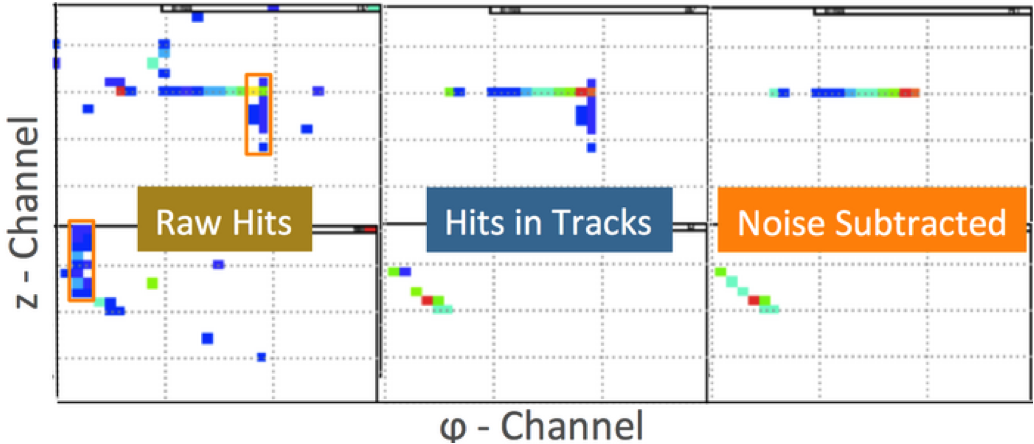
\includegraphics[width=13cm]{fig_rtpc/HotBoardSubtract.png}
  \caption{Example effects of readout board noise subtraction for tracks in two events (corresponding to the two rows in the figure).  The known hot 8x2 readout groups are shown in the orange rectange in the leftmost column.  Color scale is ADC.\label{fig:HotBoardSubtract}}
\end{figure}

\begin{figure}[htbp]\centering
  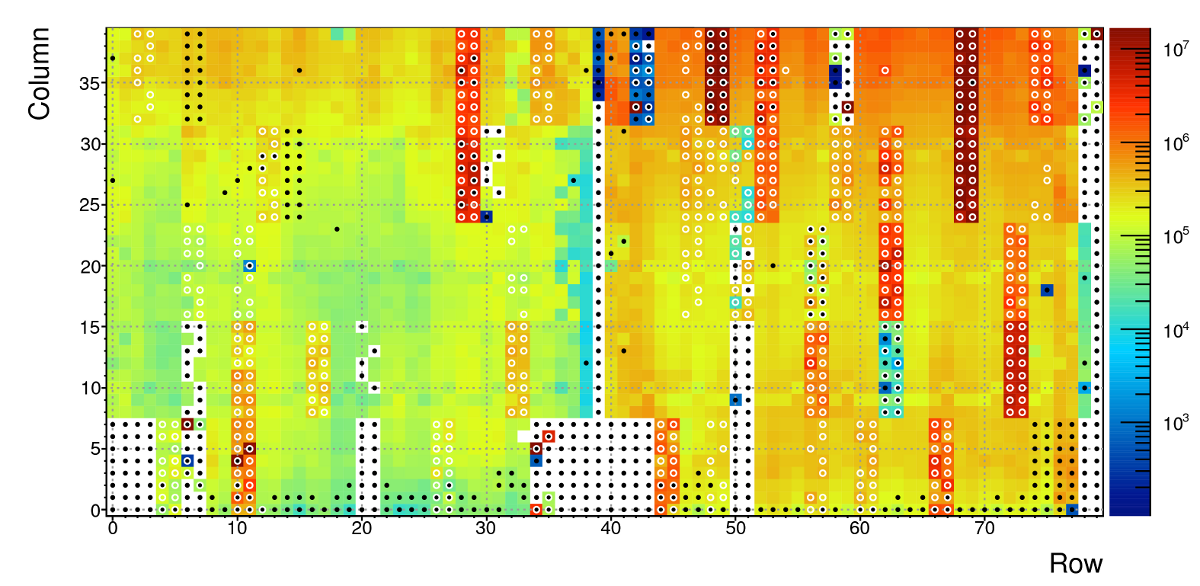
\includegraphics[width=12.3cm]{fig_rtpc/Occ2d_norej2.png}
  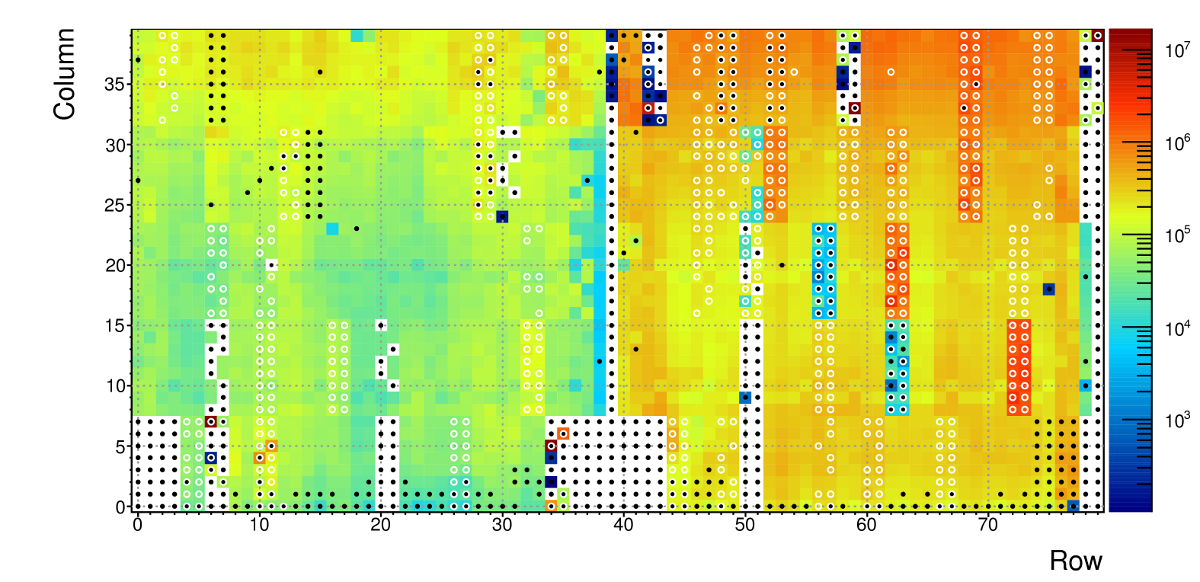
\includegraphics[width=12cm,trim={1.9cm 0 0 0},clip]{fig_rtpc/Occ2d_rej.png}
  \caption{Occupancies before (top) and after (bottom) the two noise reduction algorithms.  The event sample and occupancy color scales are identical in the two plots.\label{fig:occ_noiserej}}
\end{figure}


\clearpage
\section{Tracking resolution}
The RTPC tracking resolution is defined as the spread of the reconstructed 
track vertex, angles and momentum with respect to their true values. In the EG6 
experiment, we use the cleanly identified elastic events to estimate the RTPC 
resolutions. The CLAS detector nominally provides electron detection with an 
angular resolution around 1 and 4 mrad in $\theta$ and $\phi$, and a momentum 
resolution ($\frac{\Delta p}{p}$) around 0.5$\%$ \cite{CLASref}. The z-vertex 
resolution is about 3 mm for an extended target in the presence of the 
solenoid, as can be observed experimentally from the target window, figure 
\ref{fig:electron_z_vertex_res}. 
\begin{figure}[tbp]
   \centering
   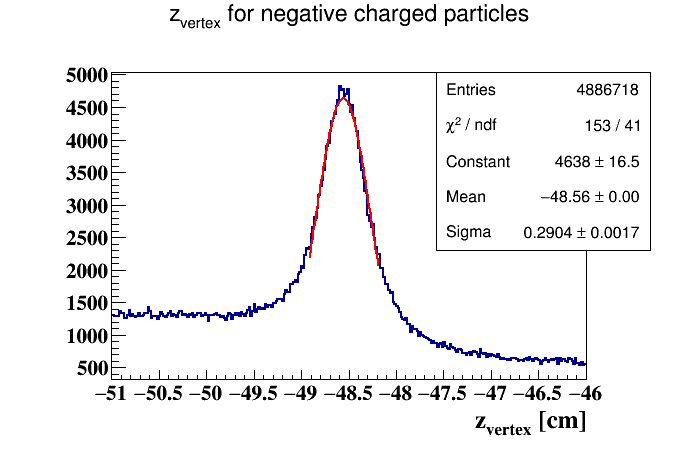
\includegraphics[height=6.2cm]{fig_rtpc/clas_z_resolution.png}
   \caption{ z-vertex of scattered electrons from the downstream window of the 
   target. The z-vetex resolution of CLAS here is about 3 mm.}
   \label{fig:electron_z_vertex_res}
\end{figure}

With such electron resolutions, one can extract the RTPC resolutions by 
comparing the calculated kinematics of the recoil elastic $^4He$ nuclei  with 
the measured experimental values, as shown in figures 
\ref{fig:rtpc_resolution_z}, \ref{fig:rtpc_resolution_phi}, 
\ref{fig:rtpc_resolution_theta}, \ref{fig:rtpc_resolution_p} for the two halves 
of the RTPC separately. The distributions are fitted with a Gaussian and the 
extracted widths are listed in table \ref{table:rtpc_resolutions}.  One can see 
that for the resolution, the two modules of the RTPC show almost the same 
performance. These resolutions will be used to match the simulated data to the 
experimental ones, as will be shown in the following chapter.

One notices slight shifts in $\Delta z$, $\Delta \phi$, and $\Delta \theta$ distributions. The reason of the shifts may rise from our non-perfect knowledge of the exact conditions in the chamber, such as the magnetic field, that affect the reconstructed parameters of the tracks. The reconstructed momenta show 10-15$\%$ systematic shifts compared to the calculated values.

\begin{figure}[tbp]
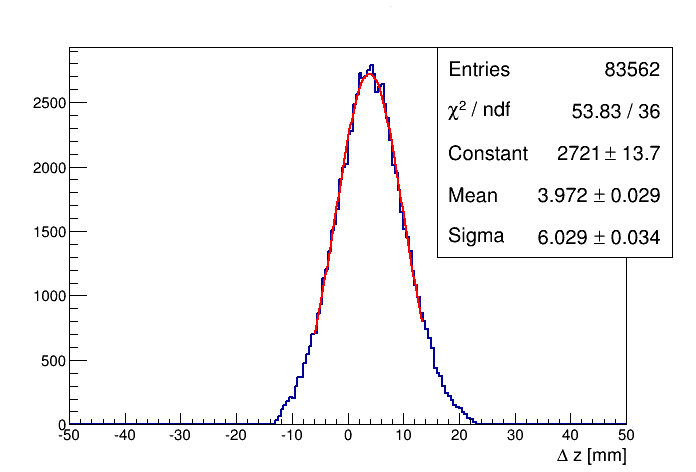
\includegraphics[scale=0.31]{fig_rtpc/fit_delta_z_l.png}
\includegraphics[scale=0.31]{fig_rtpc/fit_delta_z_r.png}
\caption{The z-vertex resolution of the two modules of the RTPC, respectively.}
\label{fig:rtpc_resolution_z}
\end{figure}

\begin{figure}[tbp]
\includegraphics[scale=0.31]{fig_rtpc/fit_delta_phi_l.png}
\includegraphics[scale=0.31]{fig_rtpc/fit_delta_phi_r.png}
\caption{The azimuthal angle resolution of the two modules of the RTPC, 
respectively.}
\label{fig:rtpc_resolution_phi}
\end{figure}

\begin{figure}[tbp]
\includegraphics[scale=0.31]{fig_rtpc/fit_delta_theta_l.png}
\includegraphics[scale=0.31]{fig_rtpc/fit_delta_theta_r.png}
\caption{The polar angle resolution of the two modules of the RTPC, 
respectively.}
\label{fig:rtpc_resolution_theta}
\end{figure}

\begin{figure}[tbp]
\includegraphics[scale=0.31]{fig_rtpc/fit_delta_p_l.png}
\includegraphics[scale=0.31]{fig_rtpc/fit_delta_p_r.png}
\caption{The momentum resolution of the two modules of the RTPC, respectively.}
\label{fig:rtpc_resolution_p}
\end{figure}
 
\begin{table}[tbp]
\begin{center}
\begin{tabular}{|l|l|l|l|l|}
\hline
RTPC's module & ~~~~~~$\sigma_{z}$ ~~~~~~&  ~~~~~~$\sigma_{\phi}$~~~~~~ & ~~~~~~$\sigma_{\theta}$~~~~~~ & ~~~~~~$\sigma_{p}$~~~~~~\\
\hline
Left module &  ~~~~6.03 mm & ~~~~1.93$^{\circ}$ & ~~~~3.78$^{\circ}$ & ~~~~~~9$\%$ \\
\hline
Right module & ~~~~7.40 mm & ~~~~1.94$^{\circ}$ & ~~~~4.02$^{\circ}$  & ~~~~~~8 $\%$\\
\hline
\end{tabular}
\caption{The resolutions of the two modules of the RTPC.}
\label{table:rtpc_resolutions}
\end{center}
\end{table}


\section{RTPC efficiency}
The previous distributions have shown that the two modules of the RTPC have 
slightly different yield, however this yield should not be linked to a different 
performance of the RTPC. The differences are mainly due to complicated 
convolution of CLAS and the RTPC acceptance. We measured the efficiency of the 
RTPC using the elastic scattering, and a result found that the left and the 
right modules have similar efficiencies except near the target windows, as 
shown in figure \ref{fig:rtpc_eff}.

\begin{figure}[tbp]
\centering
\hspace{+0.3in}\includegraphics[width=10.5cm]{fig_rtpc/tpceffyields.png}
\includegraphics[width=10cm]{fig_rtpc/tpceff.png}
\caption{On top is the inclusive and exclusive elastic yields separated into
 the two RTPC halves (LEFT/RIGHT).  Here the inclusive yields are the
 number of electrons in the elastic W-peak
 whose corresponding elastically scattered $^4$He would have been in the
 acceptance of the RTPC, and the exclusive yields require the additional
 detection of the $^4$He. On
 bottom is the RTPC $^4$He efficiency calculated from the ratio of exclusive
 and inclusive elastic yields.
 \label{fig:rtpc_eff}}
 \end{figure}


